\documentclass[11pt,a4paper]{article}

\usepackage[english]{babel}
\usepackage[utf8]{inputenc}
\usepackage[T1]{fontenc}
\usepackage{lmodern}
\usepackage[final,protrusion=true,expansion=true]{microtype}
\usepackage{textcomp}
\renewcommand{\bfdefault}{b}


\newcommand{\bn}[2]{\emph{#2}}

\usepackage{amsmath,amssymb,amsthm,mathtools}
\usepackage{bm}

\usepackage[a4paper,
            top=1.7cm, bottom=1.7cm,
            left=2.0cm, right=2.0cm,
            headheight=14pt, headsep=12pt, footskip=22pt]{geometry}
\renewcommand{\topfraction}{0.92}
\renewcommand{\bottomfraction}{0.7}
\renewcommand{\textfraction}{0.08}
\renewcommand{\floatpagefraction}{0.85}

\usepackage{setspace}
\setstretch{1.0}

\usepackage{parskip}
\setlength{\parskip}{0.35em plus 0.1em}

\usepackage{xcolor}
\definecolor{accent}{RGB}{30,72,128}
\definecolor{accent2}{RGB}{120,30,40}
\definecolor{abstractbg}{RGB}{242,242,244}
\definecolor{abstractrule}{RGB}{200,200,206}
\definecolor{tablerow}{RGB}{246,246,249}
\definecolor{capgrey}{RGB}{60,60,60}

\usepackage{fancyhdr}
\pagestyle{fancy}
\fancyhf{}
\renewcommand{\headrulewidth}{0.4pt}
\renewcommand{\footrulewidth}{0pt}
\fancyhead[L]{\small\itshape S.\,Alam, N.\,Parvez, A.\,F.\,M.\,M.\,Rahman}
\fancyhead[R]{\small\itshape BanglaCyberBench}
\fancyfoot[C]{\thepage}

\fancypagestyle{firstpage}{%
  \fancyhf{}%
  \renewcommand{\headrulewidth}{0pt}%
  \fancyfoot[C]{\thepage}%
}

\usepackage[explicit]{titlesec}
\titleformat{\section}[block]
  {\large\bfseries\color{accent}\sffamily}
  {\thesection.}{0.5em}{#1}[\vspace{-0.3em}{\color{abstractrule}\rule{\linewidth}{0.4pt}}]
\titleformat{\subsection}[block]
  {\normalsize\bfseries\sffamily}
  {\thesubsection}{0.5em}{#1}
\titleformat{\subsubsection}[block]
  {\normalsize\bfseries\sffamily\itshape}
  {\thesubsubsection}{0.5em}{#1}
\titlespacing*{\section}{0pt}{1.0em}{0.4em}
\titlespacing*{\subsection}{0pt}{0.6em}{0.2em}
\titlespacing*{\subsubsection}{0pt}{0.7em}{0.2em}

\usepackage{graphicx}
\graphicspath{{figures/}}
\usepackage{booktabs}
\usepackage{multirow}
\usepackage{makecell}
\usepackage{array}
\usepackage{tabularx}
\usepackage{colortbl}
\arrayrulecolor{black!75}
\renewcommand{\arraystretch}{1.0}
\usepackage{caption}
\captionsetup{font={small,color=capgrey},labelfont={bf,color=accent},
              labelsep=period,skip=3pt,
              justification=justified,singlelinecheck=false}
\usepackage{subcaption}
\usepackage{float}

\usepackage{algorithm}
\usepackage{algpseudocode}

\usepackage[colorlinks=true,
            linkcolor=accent,
            citecolor=accent,
            urlcolor=accent,
            filecolor=accent,
            bookmarksopen=true]{hyperref}
\usepackage[capitalise]{cleveref}
\crefname{figure}{Fig.}{Figs.}
\Crefname{figure}{Fig.}{Figs.}
\crefname{table}{Table}{Tables}
\Crefname{table}{Table}{Tables}
\crefname{equation}{Eq.}{Eqs.}
\Crefname{equation}{Eq.}{Eqs.}
\crefname{section}{Section}{Sections}
\Crefname{section}{Section}{Sections}
\crefname{algorithm}{Algorithm}{Algorithms}
\Crefname{algorithm}{Algorithm}{Algorithms}

\pdfstringdefDisableCommands{%
  \def\dset#1{#1}%
  \def\citet#1{[#1]}%
  \def\citep#1{[#1]}%
  \def\Cref#1{Section}%
  \def\cref#1{section}%
  \def\texttt#1{#1}%
  \def\textsc#1{#1}%
  \def\emph#1{#1}%
  \def\bfseries{}%
  \def\sffamily{}%
  \def\itshape{}%
}

\usepackage[numbers,square,sort&compress]{natbib}
\bibliographystyle{IEEEtranN}
\setlength{\bibsep}{1pt plus 0.5pt}

\usepackage{enumitem}
\setlist{itemsep=2pt,topsep=3pt,parsep=0pt}
\usepackage{url}
\usepackage{ragged2e}

\usepackage[most]{tcolorbox}
\newtcolorbox{journalabstract}{
  enhanced,
  colback=abstractbg,
  colframe=abstractrule,
  boxrule=0.4pt,
  arc=2pt,
  left=10pt,right=10pt,top=7pt,bottom=7pt,
  fontupper=\small,
  before skip=8pt,after skip=8pt,
}

\renewcommand{\footnoterule}{\noindent\rule{0.4\linewidth}{0.4pt}\vspace{2pt}}

\providecommand{\dset}[1]{\textsc{#1}}
\newcommand{\bench}{BanglaCyberBench}

\newcommand{\repourl}{https://github.com/Sefayet-Alam/BanglaCyberBench}

\begin{document}

\thispagestyle{firstpage}

\vspace{0.5em}
{\RaggedRight\sffamily\bfseries\Large\color{black}%
\bench{}: A Dual-Script Benchmark and a Script-Aware\\[1pt]
Ensemble for Bengali Cyberbullying Detection\par}
\vspace{0.6em}

{Sefayet Alam\textsuperscript{1,$\ast$},\quad
Naim Parvez\textsuperscript{1},\quad
A.\,F.\,M.~Minhazur Rahman\textsuperscript{1}\par}
\vspace{0.3em}

{\textsuperscript{1}Department of Computer Science and Engineering,
Rajshahi University of Engineering \& Technology (RUET), Rajshahi-6204, Bangladesh\par}
\vspace{0.2em}

{\small\textsuperscript{$\ast$}\textbf{Corresponding author:} Sefayet Alam;
\href{mailto:sefayetalam14@gmail.com}{\texttt{sefayetalam14@gmail.com}}\par}

\vspace{0.5em}
{\color{abstractrule}\rule{\linewidth}{0.4pt}}
\vspace{0.3em}

\begin{journalabstract}
\noindent\textbf{Abstract.\;}%
Bengali harmful-language classifiers are usually evaluated on a random split of one source written in one script, which gives little evidence about behaviour on data collected elsewhere. We present \bench{}, a four-source benchmark for five-class harmful-language classification in Bangla and Romanized Bangla, and we evaluate a script-aware ensemble trained with cross-entropy and the Fast Gradient Method (FGM). On the in-domain test split the ensemble reaches a Macro-F1 of 0.8225, with a 95\% bootstrap confidence interval of $[0.8146,\ 0.8300]$. Macro-F1 is 0.8303 for Bangla-script comments and 0.3900 for Romanized comments under the fixed five-class definition. The supported-class Macro-F1 for Romanized comments is 0.4875, because the Romanized test subset contains no \emph{threat} examples. Source-held-out Macro-F1 ranges from 0.4612 to 0.5850, so performance falls when the test source is unseen during training. The labels type the harmful content of an isolated comment rather than cyberbullying in its interactional sense of repetition, power imbalance, or victim history, none of which the comment-level sources record.

\vspace{4pt}
\noindent\textbf{Keywords:}\; Bengali harmful-language detection;\; Romanized Bangla;\; dual-script benchmark;\; script-aware ensemble;\; adversarial fine-tuning;\; class imbalance;\; cross-source generalisation.
\end{journalabstract}

\vspace{0.2em}

\section{Introduction}
\label{sec:introduction}

Bengali harmful-language detection has to account for two written forms. Bengali is spoken by more than 240 million people, and a large share of its social-media text is typed in the Latin alphabet rather than in Bangla script. The Romanized form \emph{tui akta faltu manush} and its Bangla-script equivalent carry the same insult in two different surfaces. Existing Bengali datasets differ in source, script, and label definition, which makes direct comparison difficult and complicates transfer between them.

Most prior studies report random within-dataset evaluation. Such evaluation does not measure performance on a new source, and cross-dataset degradation is already well established in abusive-language detection \citep{arango2019validation,swamy2019generalisability,wiegand2019biased,fortuna2021generalize,yin2021generalisable}. The published comparator for this study reports a Weighted-F1 of 0.8923 and a Macro-F1 of 0.8803 on its single-source protocol \citep{hoque2025transformerstacking}. We therefore treat source-held-out evaluation as a Bengali replication and quantification of a known problem rather than as the discovery of source shift.

We address three research questions. \textbf{RQ1} (\cref{sec:benchmark}) evaluates whether four Bengali sources can be mapped to a shared five-class taxonomy. \textbf{RQ2} (\cref{sec:main-results,sec:perclass-results,sec:scriptmask-results}) measures in-domain and script-stratified performance of a script-aware ensemble. \textbf{RQ3} (\cref{sec:ablation-results,sec:robustness-results}) evaluates component sensitivity and source-held-out generalisation under the retained protocol.

\subsection{Contributions}
\label{sec:contributions}

\textbf{(C1) Shared benchmark protocol.} We map four Bengali harmful-language datasets to a common five-class taxonomy, preserve script information, and construct random and source-held-out evaluation protocols. The merged corpus contains 94{,}323 comments after exact-text deduplication, 60.4\% in Bangla script and 39.6\% Romanized.

\textbf{(C2) Script-aware reference model.} We evaluate an ensemble of Bangla, bilingual, and multilingual encoders trained with cross-entropy and FGM. BanglaBERT is excluded from Romanized inputs according to its pretraining scope.

\textbf{(C3) Multi-level evaluation.} We report in-domain, per-class, script-stratified, component, taxonomy, and source-held-out results. Bootstrap confidence intervals are reported where the required predictions are available.

\textbf{(C4) Evaluation findings.} The experiments quantify cross-source degradation and report script-stratified performance together with the support of each class.

The proposed model is offered as the fully specified reference system that the protocol needs, not as an algorithmic novelty claim. Pretrained encoders, FGM, and weighted fusion are all established components. The new material is the consolidated resource, the evaluation protocol applied to it, and the measurements that protocol produces.

The rest of the paper is organised as follows. \Cref{sec:related-work} reviews prior work. \Cref{sec:benchmark} describes the benchmark and its construction. \Cref{sec:methodology} formalises the proposed model on a single comment. \Cref{sec:setup} gives the experimental setup. \Cref{sec:results} reports results. \Cref{sec:discussion} discusses the findings and their limitations, and \cref{sec:conclusion} concludes.

\section{Related Work}
\label{sec:related-work}

\subsection{Bengali Cyberbullying and Hate-Speech Detection}
\label{sec:rw-bengali}

Earlier Bengali harmful-language studies evaluated classical classifiers, neural sequence models, and transformer encoders, usually on one dataset \citep{ahmed2021deployment,romim2021hate,karim2021deephateexplainer,akhter2023robust}. TF-IDF features with logistic regression, support vector machines, and tree ensembles were common in the earliest work \citep{ahmed2021deployment,akhter2023robust,saha2023bengali}, and BiLSTM and CNN-BiLSTM models with FastText or GloVe embeddings followed \citep{romim2021hateban,nath2024deeplearning}. Transformer encoders are now the usual choice. \citet{emon2022detection} and \citet{aurpa2022abusive} applied BERT-family encoders to Bangla abusive-comment detection, \citet{karim2021deephateexplainer} added explainability to Bengali hate-speech classification, and \citet{saifullah2024cyberbullying} combined deep learning with transformer language models. Recent transformer-based systems improve in-domain performance, but most do not evaluate transfer to an unseen source. The comparator used in this study evaluates a transformer ensemble on Facebook-44K under a single-source protocol \citep{hoque2025transformerstacking}. That protocol does not measure cross-source transfer and does not use FGM, so our FGM result is a property of the proposed training configuration rather than a claim about the comparator.

Bengali resources have grown alongside the methods. \citet{romim2021hate} released a Bengali hate-speech corpus with baseline evaluation, and \citet{ahmed2021bangla} built a Facebook harassment dataset with exploratory analysis. Regional and multi-task resources such as BIDWESH \citep{gomes2025bidwesh} and LLM-based multi-task hate-speech corpora \citep{banglamultihate2025} extend coverage to dialects and severity. BanTH \citep{haider2025banth}, a large transliterated-Bangla dataset and one of the four sources consolidated here, and BanCyB \citep{hasan2026bancyb} broaden the field further. Our claim is therefore scoped to this consolidated benchmark and its evaluation protocol rather than to Bengali harmful-language detection in general. \Cref{tab:priordata} places \bench{} against representative prior resources on the axes that matter for this paper: number of sources, script coverage, taxonomy granularity, and whether transfer to an unseen distribution was measured.

\begin{table}[!htbp]
\centering
\caption{Representative Bengali abuse-detection resources against \bench{}. ``Shift tested'' asks whether the study measured transfer to an unseen source or script rather than only a random in-domain split.}
\label{tab:priordata}
\small
\begin{tabularx}{\textwidth}{@{}lcccc>{\raggedright\arraybackslash}X@{}}
\toprule
\textbf{Resource} & \textbf{Sources} & \textbf{Script} & \textbf{Classes} & \textbf{Shift tested} & \textbf{Size} \\
\midrule
Romim et al.\ \citep{romim2021hate} & 1 & Bangla & binary & no & 30k \\
Ahmed et al.\ \citep{ahmed2021deployment} & 1 & Bangla + Rom. & binary & no & 12k \\
Karim et al.\ \citep{karim2021deephateexplainer} & 1 & Bangla & 4 & no & 8{,}087 \\
Base paper \citep{hoque2025transformerstacking} & 1 & Bangla & 5 & no & 44{,}001 \\
\textbf{\bench{} (ours)} & \textbf{4} & \textbf{Bangla + Rom.} & \textbf{5} & \textbf{yes} & \textbf{94{,}323} \\
\bottomrule
\end{tabularx}
\end{table}

\subsection{Cross-Dataset Generalisation}
\label{sec:rw-crossdataset}

Cross-dataset degradation is a recurring result in abusive-language detection. Prior work attributes it to dataset-specific sampling, annotation policy, topic distribution, and differences in the label space \citep{arango2019validation,swamy2019generalisability,wiegand2019biased,fortuna2021generalize}. \citet{yin2021generalisable} review these obstacles and the mitigation strategies proposed for them. Our contribution is a Bengali, dual-script quantification under a fixed source-held-out protocol, not the first observation that random-split performance transfers poorly.


\subsection{Romanized Bangla and the Script Problem}
\label{sec:rw-script}

Romanized Bangla is non-standardised and frequently code-mixed with English, and it drops vowels freely. \citet{ahmed2021deployment} is one of the few Bengali studies to treat both scripts side by side, and it does so with classical models on a modest scale. TB-OLID provides a directly relevant offensive-language benchmark for transliterated and code-mixed Bangla \citep{raihan2023tbolid}, BanglaTLit provides back-transliteration pairs \citep{fahim2024banglatlit}, and BanTH provides a Romanized Bengali harmful-language resource \citep{haider2025banth}. The available pretrained encoders divide along the same line. BanglaBERT \citep{bhattacharjee2022banglabert} is an ELECTRA-style discriminator pretrained primarily on Bangla-script text. BanglishBERT is a Bangla-English bilingual encoder and is not pretrained on Romanized Bengali. MuRIL \citep{khanuja2021muril} includes transliterated Indic text in pretraining, and XLM-R \citep{conneau2020xlmr} provides a multilingual reference. Recent Bangla shared-task work also provides context for current hate-speech evaluation \citep{hasan2025blp}. Whether one encoder can serve both scripts is an open question, and the script-aware design of \cref{sec:methodology} treats it as a pretraining-scope constraint rather than a settled empirical result.

\subsection{Adversarial and Imbalance-Aware Fine-Tuning}
\label{sec:rw-methods}

Perturbing continuous word-embedding parameters during training is an inexpensive regulariser for small-data text classification. The Fast Gradient Method (FGM) \citep{miyato2017adversarial}, a text adaptation of the image-domain idea of \citet{goodfellow2015explaining}, adds one adversarial forward-backward pass per batch. Other components target class imbalance and overfitting. Focal loss \citep{lin2017focal} and class-balanced weighting \citep{cui2019classbalanced} down-weight easy majority examples. Multi-sample dropout \citep{inoue2019multisample} reduces head variance, R-Drop \citep{liang2021rdrop} enforces consistency between two dropout passes, weight averaging in the style of mean teachers \citep{tarvainen2017meanteacher} stabilises evaluation weights, and logit adjustment \citep{menon2021longtail} corrects the long tail at inference. Our fixed single-backbone sensitivity run compares these choices descriptively and does not establish a universal ordering. The proposed model uses cross-entropy with FGM as a transparent compromise between the measured differences and training cost.


\section{The \bench{} Benchmark}
\label{sec:benchmark}

\bench{} merges four public Bengali datasets into one deduplicated, dual-script, five-class corpus. \Cref{fig:pipeline} shows the construction pipeline, and this section describes each stage.

\paragraph{Task scope.} \bench{} evaluates comment-level harmful-language classification. Each isolated comment is assigned to None, Abusive, Religious, Sexual, or Threat. The data do not contain conversation history, repeated targeting, power imbalance, or victim information. The task therefore does not model cyberbullying as an interactional phenomenon, and the term is retained only for continuity with the source datasets. A title of the form ``harmonising multi-source Bengali harmful-language data'' would describe the contribution equally well.

\begin{figure}[!htbp]
\centering

\includegraphics[width=0.98\textwidth]{D1_Benchmark_Construction.png}
\caption{Benchmark construction pipeline. Four sources are mapped to a common representation, normalised, deduplicated on cleaned text ($135{,}575 \rightarrow 94{,}323$), consolidated from 89 raw label strings into five classes by a priority rule, and split into a stratified random 70/10/20 partition and three source-held-out configurations. Every configuration asserts an empty intersection of comment identifiers between training and test.}
\label{fig:pipeline}
\end{figure}

\subsection{Sources and Schema Unification}
\label{sec:sources}

The benchmark combines Facebook-44K, BanTH, Multilabel-12.5K, and the publicly available BD-SHS test partition (\cref{tab:sources}). The BD-SHS contribution contains 5{,}029 comments. We map the source texts, labels, provenance, and script information to a common representation before deduplication and splitting. BanTH supplies the Romanized comments, and the other three sources use Bangla script. BanTH is therefore the only Romanized source, which is why source-held-out evaluation on BanTH and any cross-script analysis are closely related rather than independent.

\begin{table}[!htbp]
\centering
\caption{The four sources after deduplication. BanTH is the only Romanized-Bangla source, and the other three are Bangla script. Shares are of the 94{,}323-comment benchmark.}
\label{tab:sources}
\small
\begin{tabularx}{\textwidth}{@{}lllrX@{}}
\toprule
\textbf{Source} & \textbf{Script} & \textbf{Origin} & \textbf{Samples} & \textbf{Raw label style} \\
\midrule
Facebook-44K \citep{ahmed2021bangla} & Bangla & Mendeley Data & 43{,}078 & single label column \\
BanTH \citep{haider2025banth} & Romanized & public release & 37{,}334 & binary column and per-type indicators \\
Multilabel-12.5K \citep{sunny2024multilabel} & Bangla & Mendeley Data & 8{,}882 & separate per-type indicators \\
BD-SHS (public test partition) \citep{romim2022bdshs} & Bangla & ACL repository & 5{,}029 & one harmful column and one type column \\
\midrule
\textbf{Total} & NA & NA & \textbf{94{,}323} & NA \\
\bottomrule
\end{tabularx}
\end{table}

\subsection{Preprocessing}
\label{sec:preprocessing}

Bengali harmful language relies on cues that aggressive normalisation destroys, so the cleaning is light and script-safe. We apply Unicode NFKC normalisation, remove invisible and zero-width characters, mask URLs and user mentions, preserve hashtag text, convert emoji to text tokens, collapse runs of three or more identical characters down to two, and standardise whitespace. Collapsing repeats keeps \emph{baaaaje} and \emph{baje} from being treated as unrelated. We do not case-fold beyond Unicode rules, strip punctuation, or remove stopwords, because emphatic repetition, punctuation, and emoji all carry signal and subword tokenisers handle the raw form well. The same procedure is applied before deduplication and before model input construction. \Cref{fig:composition} shows the composition of the resulting benchmark by source, script, and class.

\begin{figure}[!htbp]
\centering

\includegraphics[width=0.98\textwidth]{fig_dataset_composition_pies.png}
\caption{Composition of \bench{} after deduplication ($n = 94{,}323$). Left: the four merged sources. Middle: the split between Bangla script (60.4\%) and Romanized Bangla (39.6\%). Right: the five-class distribution, dominated by \emph{none} and \emph{abusive}, with \emph{threat} at 3.4\%.}
\label{fig:composition}
\end{figure}

\subsection{Deduplication}
\label{sec:dedup}

Records are grouped by exact normalized text before any split is drawn. The merged data contain 135{,}575 rows before exact-text deduplication and 94{,}323 retained comments afterward, so 41{,}252 rows are removed. BanTH contracts the most because it carried many near-identical scrapes, which is why its retained share is smaller than its raw size suggests. When records in one group carry conflicting labels, the fixed priority rule of \cref{eq:priority} assigns one final class, the binary flag is set if any record in the group was flagged harmful, and one representative record is retained. That record keeps the source and script of the first row in the deterministic merge order, which the benchmark treats as a primary-source field rather than an assertion about where the comment originated. Grouping before splitting prevents exact normalized duplicates from crossing partitions, and an identifier-intersection assertion after every split confirms it. Fuzzy paraphrase-level duplicates are not detected (\cref{sec:limitations}). Across the merged data, 1{,}287 groups span more than one source, covering 3{,}308 rows. Of those groups, 661 carry conflicting five-class labels over 1{,}721 rows, and 271 carry conflicting binary flags over 767 rows.

\subsection{The Five-Class Taxonomy}
\label{sec:taxonomy}

The four sources together use 89 distinct raw label strings, many of them comma- or underscore-compounded (a single comment might be tagged \texttt{sexual\_threat} or \texttt{religious,abusive}). We split each raw string on \texttt{,} and \texttt{\_}, map each piece to a bucket, and resolve compounds by a fixed priority:
\begin{equation}
\textbf{threat} \;>\; \textbf{sexual} \;>\; \textbf{religious} \;>\; \textbf{abusive} \;>\; \textbf{none}.
\label{eq:priority}
\end{equation}
Explicit violence and identity-targeted abuse take precedence over the generic \emph{abusive} bucket, and \emph{none} loses to every other class. This ordering is a benchmark-construction decision motivated by moderation urgency, not a universal semantic hierarchy, and the released code re-consolidates the data under an alternative rule. Harmonising source taxonomies is necessary because abusive-language datasets frequently use incompatible task and label definitions \citep{fortuna2020taxonomy}. Two consistency rules run alongside the priority order. An unrecognised component under a record flagged abusive is sent to \emph{abusive} rather than dropped, and the binary flag has the final say, so a record flagged non-abusive resolves to \emph{none} and one flagged abusive but resolving to \emph{none} is moved to \emph{abusive}. The resulting distribution (\cref{tab:classes}) is imbalanced, with \emph{none} at half the data and \emph{threat} at 3.4\%, a ratio of roughly 14.8:1 between the most and least frequent class.

\begin{table}[!htbp]
\centering
\caption{Class distribution of the five-class benchmark after deduplication ($n = 94{,}323$). Raw labels folded into each class are listed in the text.}
\label{tab:classes}
\small
\begin{tabular}{@{}lrr@{}}
\toprule
\textbf{Class} & \textbf{Samples} & \textbf{Share (\%)} \\
\midrule
None & 47{,}312 & 50.16 \\
Abusive & 24{,}963 & 26.47 \\
Sexual & 10{,}822 & 11.47 \\
Religious & 8{,}032 & 8.52 \\
Threat & 3{,}194 & 3.39 \\
\midrule
\textbf{Total} & \textbf{94{,}323} & \textbf{100.00} \\
\bottomrule
\end{tabular}
\end{table}

The five buckets absorb the raw strings as follows. \emph{None} folds in \texttt{none} and \texttt{not-bully}. \emph{Abusive} is the residual bucket for general offence, covering abusive or violent content, troll, personal offence, body-shaming, origin-based slurs, slander, spam, political abuse, and miscellaneous. \emph{Sexual} folds sexual and gender-based harassment, \emph{Religious} folds religion-directed abuse, and \emph{Threat} folds explicit threats and calls to violence. \Cref{tab:consolidation} gives the full map.

The five labels do not sit on a single axis. \emph{None} is a harmfulness decision, \emph{threat} marks an act, \emph{sexual} and \emph{religious} are partly target-identity categories, and \emph{abusive} is a residual content bucket. Some folds are arguable, in particular gender-based abuse under \emph{sexual} and origin-based slurs under the generic \emph{abusive} bucket. A multi-label or hierarchical representation would capture such cases more faithfully than a flat forced choice. We keep the flat rule for comparability with the source datasets and the comparator, and we do not claim it is the uniquely correct one. A sensitivity study across consolidation policies is left to future work (\cref{sec:limitations}).

Two authors independently labelled a stratified sample of 500 comments using the five-class taxonomy. The sample was drawn with a fixed seed, stratified jointly by class and script, and labelled blind to the consolidated label and to each other. They agreed on 80.0\% of the items. Cohen's $\kappa$ \citep{cohen1960kappa} was 0.7094, with a 95\% bootstrap confidence interval of $[0.6583, 0.7579]$ based on 5{,}000 resamples \citep{artstein2008intercoder} (\cref{tab:iaa}). The sample contains no Romanized Threat stratum because that combination is absent from the benchmark. Disagreements were left unadjudicated by design, since the aim was to measure convergence on the consolidated scheme rather than to build a corrected gold set. A larger study with more annotators and adjudication is future work (\cref{sec:limitations}).

\begin{table}[!htbp]
\centering
\caption{Agreement between two author-annotators on a stratified sample of 500 comments.}
\label{tab:iaa}
\small
\begin{tabular}{@{}lc@{}}
\toprule
\textbf{Measure} & \textbf{Value} \\
\midrule
Observed agreement & 80.0\% \\
Cohen's $\kappa$ & 0.7094 \\
95\% bootstrap CI & $[0.6583,\ 0.7579]$ \\
Bootstrap resamples & 5{,}000 \\
Sample size & 500 \\
\bottomrule
\end{tabular}
\end{table}

A nine-class variant that splits the residual bucket further, adding \texttt{personal}, \texttt{political}, \texttt{gender}, and \texttt{other}, is built only for the taxonomy sensitivity analysis of \cref{sec:ablation-results} and never for the headline result.

\begin{table}[!htbp]
\centering
\caption{Raw-label consolidation map. Each raw label string is lowercased and split on \texttt{,} and \texttt{\_}; every component is sent to a bucket, and compounds are resolved by the priority order in \cref{eq:priority}.}
\label{tab:consolidation}
\small
\begin{tabularx}{\textwidth}{@{}lX@{}}
\toprule
\textbf{Consolidated class} & \textbf{Raw components folded in} \\
\midrule
None & \texttt{none}, \texttt{not bully}, \texttt{notbully} \\
Abusive & \texttt{abusive}, \texttt{abusive/violence}, \texttt{violence}, \texttt{troll}, \texttt{personal}, \texttt{personal offense}, \texttt{political}, \texttt{slander}, \texttt{spam}, \texttt{origin}, \texttt{body shaming}, \texttt{misc} \\
Sexual & \texttt{sexual}, \texttt{gender} \\
Religious & \texttt{religious}, \texttt{religion} \\
Threat & \texttt{threat}, \texttt{calltoviolence} \\
\bottomrule
\end{tabularx}
\end{table}

\subsection{Splits and Evaluation Protocol}
\label{sec:splits}

We report two protocols. The in-domain protocol uses a group-stratified 70/10/20 split of the combined benchmark, giving 66{,}026 training, 9{,}432 validation, and 18{,}865 test comments (\cref{tab:split}). Stratification holds the five-class proportions fixed across the three partitions, so the rare \emph{threat} and \emph{religious} classes keep the same share in each. The validation split is used for early stopping, model selection within a run, the fusion weights of \cref{eq:weightopt}, and any inference-time tuning. No hyperparameter, checkpoint, or fusion weight of the final model is chosen using test data. The random split measures generalisation to unseen comments from the same consolidated mixture, not generalisation to a new platform. The component and routing analyses of \cref{sec:ablation-results,sec:scriptmask-results} also report test-split scores so that they use the same measurement as the headline. The proposed configuration was fixed before those tables were assembled, and they should be read as reported measurements rather than as the selection procedure.

The source-held-out protocol evaluates each of the three Bangla-script sources as the complete test set while splitting the other two into training and validation sets by a stratified 87.5/12.5 partition. BanTH is not included in this protocol because it supplies the benchmark's Romanized data, and it remains part of the in-domain benchmark. Holding BanTH out would remove every Romanized comment from training and test only on Romanized text, so the resulting score would confound source shift with script shift. Separating the two effects requires a second Romanized source, which we identify as the benchmark's most useful extension (\cref{sec:limitations}).

Two further properties of the protocol are worth stating. The script tag $s(x)$ used throughout the paper is inherited from source provenance rather than detected per comment, which is exact here because each source is script-homogeneous. Because global deduplication attributes text shared across sources to a single primary source, a held-out test set contains the benchmark rows tagged with that source rather than a from-scratch reconstruction of the source as originally collected. The 1{,}287 groups that span multiple sources therefore sit in training under whichever source they were first attributed to. Of those, 661 carry conflicting five-class labels, so the net effect on transfer difficulty is not signed in one direction. The two split manifests correspond to the in-domain and Bangla-script source-held-out protocols, respectively, and every configuration re-runs the identifier-intersection assertion, so no retained comment appears in more than one partition.

\begin{table}[!htbp]
\centering
\caption{Stratified random 70/10/20 split of the benchmark. Stratification is on the five-class label.}
\label{tab:split}
\small
\begin{tabular}{@{}lrr@{}}
\toprule
\textbf{Split} & \textbf{Samples} & \textbf{Share (\%)} \\
\midrule
Train & 66{,}026 & 70.00 \\
Validation & 9{,}432 & 10.00 \\
Test & 18{,}865 & 20.00 \\
\bottomrule
\end{tabular}
\end{table}

\section{Proposed Model}
\label{sec:methodology}

The proposed model combines four transformer encoders using script-dependent activation and validation-selected logit fusion. Each encoder uses the same pooling head and is trained with cross-entropy and FGM. BanglaBERT is active only for Bangla-script comments, and the other three encoders process both script subsets. This section follows a single comment through the system: tokenisation and encoding (\cref{sec:prelim}), the pooling and classification head (\cref{sec:head}), the training objective (\cref{sec:objective}), the script-dependent activation rule (\cref{sec:scriptaware}), and the weighted-logit fusion that produces the final label (\cref{sec:fusion}). \Cref{fig:ensemble} shows the assembled system, and \cref{tab:notation} fixes notation.

\begin{figure}[!htbp]
\centering
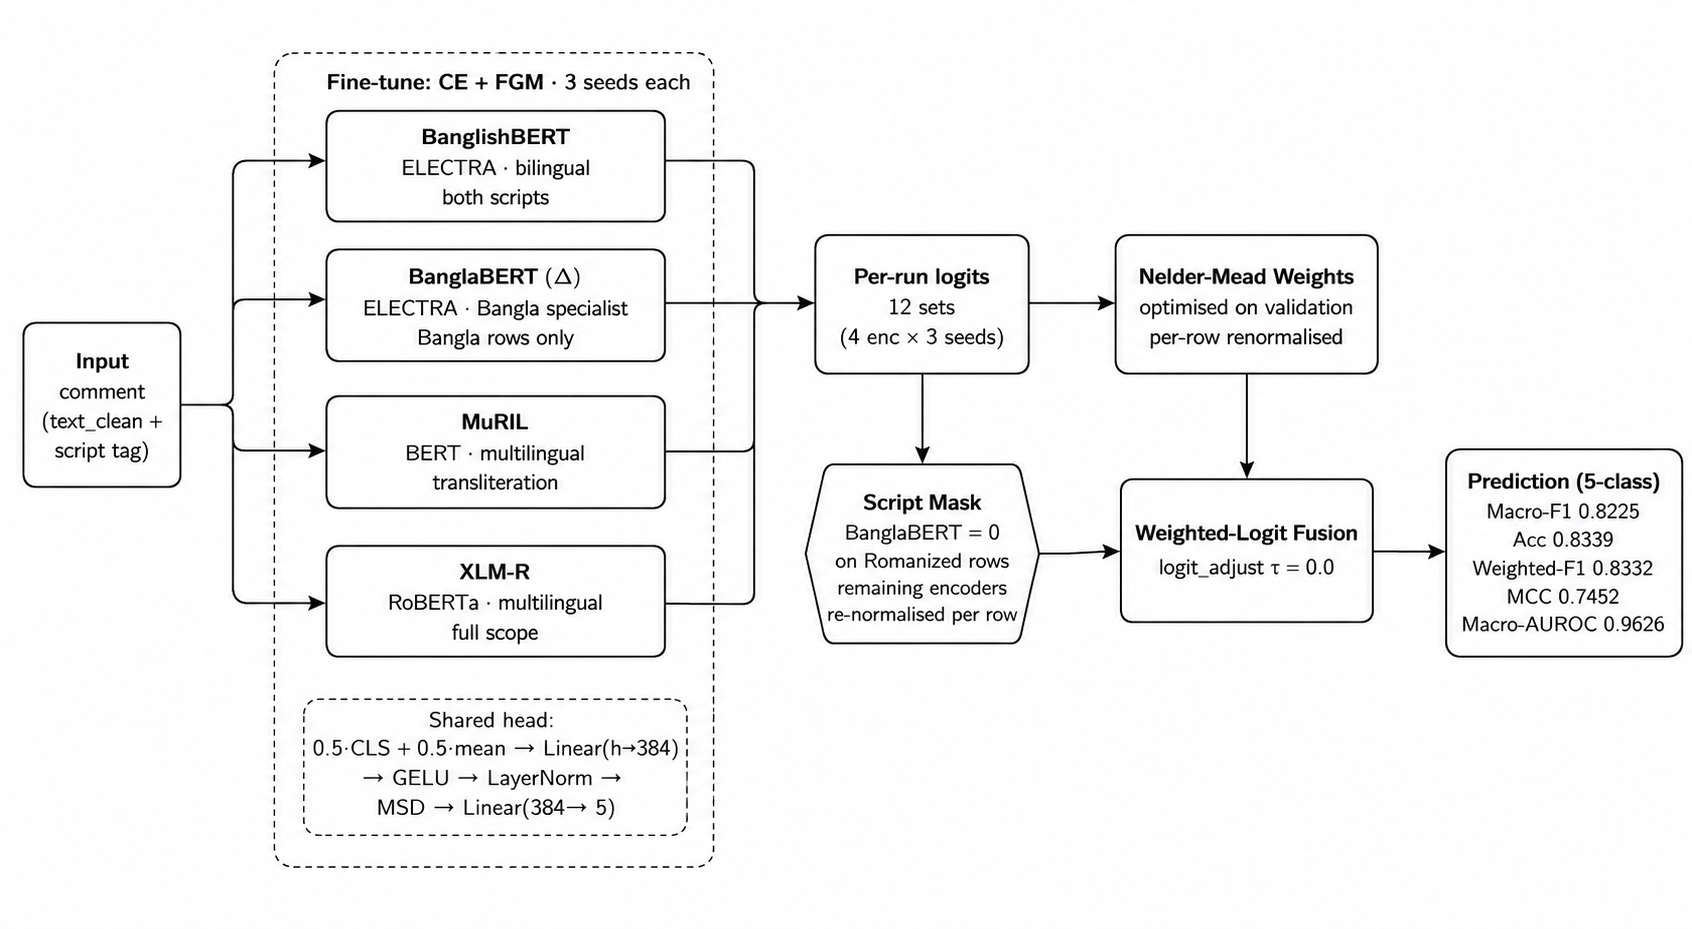
\includegraphics[width=1.0\textwidth]{D2_Script_Aware_Ensemble.png}
\caption{The proposed script-aware ensemble. All four encoders process Bangla-script comments. On Romanized comments BanglaBERT emits neutral logits and receives zero fusion weight, so the remaining encoders decide the label. Each encoder is fine-tuned with cross-entropy and FGM across three seeds, and the twelve resulting logit vectors are fused by validation-selected weights.}
\label{fig:ensemble}
\end{figure}

\begin{table}[!htbp]
\centering
\caption{Notation used in \cref{sec:methodology}.}
\label{tab:notation}
\small
\begin{tabularx}{\textwidth}{@{}lX@{}}
\toprule
\textbf{Symbol} & \textbf{Meaning} \\
\midrule
$x$, $y$ & Input comment (token sequence) and its ground-truth class \\
$T$, $C$ & Sequence length ($\le 128$ tokens) and number of classes ($C = 5$) \\
$s(x) \in \{\textsc{bn}, \textsc{rom}\}$ & Script of comment $x$: Bangla or Romanized \\
$N_b$, $N_{\mathrm{test}}$ & Minibatch size and number of test comments \\
$\theta_m$, $\phi_m$ & Encoder and head parameters of backbone $m$ \\
$\mathbf{h}_t \in \mathbb{R}^{d}$ & Contextual hidden state at position $t$, of width $d = 768$; $\mathbf{h}_{[\mathrm{CLS}]} \equiv \mathbf{h}_0$ \\
$a_t \in \{0,1\}$ & Attention-mask entry indicating a non-padding position \\
$\alpha_m(x) \in \{0,1\}$ & Activation indicator of member $m$ on comment $x$ \\
$\mathbf{z}_m \in \mathbb{R}^{C}$ & Logit vector from backbone $m$ \\
$\hat{p}(y \mid x) \in \Delta^{C-1}$ & Predicted class-probability vector \\
$\mathbf{E}_m$, $\mathbf{r}$ & Token-embedding parameter of member $m$ and its temporary FGM perturbation \\
$\epsilon$ & FGM perturbation budget \\
$w_m \ge 0$ & Fusion weight of ensemble member $m$, $\sum_m w_m = 1$ \\
$\mathcal{M}$, $\mathcal{M}(x)$ & Full member set (12) and the active members for comment $x$ \\
\bottomrule
\end{tabularx}
\end{table}

\subsection{From a Comment to Contextual Embeddings}
\label{sec:prelim}

Each tokenizer truncates or pads a comment to $T \le 128$ subword tokens, with a leading \texttt{[CLS]} and a trailing \texttt{[SEP]}. The corresponding unmodified 12-layer transformer backbone \citep{vaswani2017attention} produces contextual hidden states $(\mathbf{h}_0,\ldots,\mathbf{h}_{T-1})$ of width $d = 768$, whose parameters we write as the encoder set $\theta_m$. All backbone parameters are fine-tuned jointly with the pooling and classification head described below.

Two of the backbones, BanglaBERT and BanglishBERT \citep{bhattacharjee2022banglabert}, are pretrained as ELECTRA discriminators \citep{clark2020electra} rather than as masked language models. MuRIL and XLM-R are masked-language-model encoders. The pretraining objective matters here only through the representations it produces, and the fine-tuning path below is identical across all four.

\subsection{Pooling and Classification Head}
\label{sec:head}

Each backbone $m$ carries the same head. The sequence is pooled by an equal-weight blend of the \texttt{[CLS]} vector and a mean over token states:
\begin{equation}
\mathbf{h}_{\mathrm{pool}} = \tfrac{1}{2}\,\mathbf{h}_{[\mathrm{CLS}]} + \tfrac{1}{2}\cdot\frac{\sum_{t=1}^{T} a_t\,\mathbf{h}_t}{\sum_{t=1}^{T} a_t},
\label{eq:pool}
\end{equation}
where $a_t \in \{0,1\}$ is the attention-mask entry that zeroes out padding, and $m$ indexes an ensemble member. The pooled vector passes through a small projection with GELU and layer normalisation, then a linear layer to $C$ logits:
\begin{equation}
\mathbf{u} = \mathrm{LN}\!\big(\mathrm{GELU}(\mathbf{W}_1 \mathbf{h}_{\mathrm{pool}} + \mathbf{b}_1)\big) \in \mathbb{R}^{384},
\qquad
\mathbf{z}_m = \mathbf{W}_2\,\mathbf{u} + \mathbf{b}_2 \in \mathbb{R}^{C},
\label{eq:head}
\end{equation}
with $\mathbf{W}_1 \in \mathbb{R}^{384 \times d}$ and $\mathbf{W}_2 \in \mathbb{R}^{C \times 384}$. The class probabilities are $\hat{p}(y \mid x) = \mathrm{softmax}(\mathbf{z}_m)$. The equal-weight pooling blend and the label-smoothing value defined below are fixed configuration choices. They were not optimized and are not evaluated in a separate ablation.

\subsection{Training Objective: Cross-Entropy with FGM}
\label{sec:objective}

Each backbone is fine-tuned end to end, over both $\theta_m$ and $\phi_m$, with AdamW \citep{loshchilov2019adamw} under label-smoothed cross-entropy \citep{szegedy2016labelsmoothing}. With smoothing $s = 0.03$ the soft target is $\tilde{y}_c = (1-s)\,\mathbb{1}[c = y] + s/C$, and
\begin{equation}
\mathcal{L}_{\mathrm{CE}}(\theta_m, \phi_m) = -\frac{1}{N_b}\sum_{i=1}^{N_b}\sum_{c=1}^{C} \tilde{y}_{i,c}\,\log \hat{p}(y = c \mid x_i).
\label{eq:ce}
\end{equation}
Adversarial training adds a second pass in which the input embeddings are perturbed in the direction that most increases the loss. Written as a min-max problem,
\begin{equation}
\min_{\theta_m, \phi_m}\; \mathbb{E}_{(x,y)}\Big[\max_{\|\mathbf{r}\|_F \le \epsilon}\; \mathcal{L}_{\mathrm{CE}}\big(\mathbf{E}_m + \mathbf{r};\,x,y\big)\Big].
\label{eq:minmax}
\end{equation}
FGM \citep{miyato2017adversarial} is implemented here as a temporary perturbation of the trainable token-embedding parameter, rather than as a persistent change to the input ids. Let $\mathbf{E}_m$ denote the token-embedding parameter of backbone $m$ and let $\mathbf{g}_{E}=\nabla_{\mathbf{E}_m}\mathcal{L}_{\mathrm{CE}}(\mathbf{E}_m,y)$ be its clean-pass gradient. A first-order Taylor expansion gives $\mathcal{L}_{\mathrm{CE}}(\mathbf{E}_m+\mathbf{r}, y) \approx \mathcal{L}_{\mathrm{CE}}(\mathbf{E}_m,y)+\langle\mathbf{r},\mathbf{g}_{E}\rangle_F$, so the inner problem under a Frobenius-norm budget is maximised by
\begin{equation}
\boxed{\;\mathbf{r}_{\mathrm{adv}} = \epsilon\,\frac{\mathbf{g}_{E}}{\|\mathbf{g}_{E}\|_F}\;}
\label{eq:fgm}
\end{equation}
a single ascent step on the embedding-parameter ball. The perturbation is applied in-place to the embedding weight for the adversarial forward pass and then restored, so the optimiser never treats it as a new parameter. The per-batch objective sums the clean and adversarial forward passes,
\begin{equation}
\mathcal{L}(\theta_m, \phi_m) = \mathcal{L}_{\mathrm{CE}}(\mathbf{E}_m; x,y) + \mathcal{L}_{\mathrm{CE}}(\mathbf{E}_m + \mathbf{r}_{\mathrm{adv}}; x,y),
\label{eq:fgm-loss}
\end{equation}
and both passes accumulate gradients into the same parameters before a single optimiser step (\cref{alg:fgm}). FGM costs one extra forward-backward pass per batch and exposes a single hyperparameter $\epsilon$, fixed at $1.0$.

\paragraph{Parameter updates.} The encoder and classification head are fine-tuned jointly with AdamW \citep{loshchilov2019adamw}. For each minibatch, gradients from the clean and adversarial passes are accumulated before one optimizer update. The encoder and head use separate learning rates (\cref{tab:hparams}), gradients are clipped in $\ell_2$ norm before the update, and the learning rate is warmed up linearly and then decayed. \Cref{sec:ablation-results} reports the component sensitivity analysis that motivates using FGM without additional regularisation.

\begin{algorithm}[!htbp]
\caption{Cross-entropy $+$ FGM fine-tuning of one backbone (single mini-batch).}
\label{alg:fgm}
\begin{algorithmic}[1]
\Require Batch $(x, y)$, encoder $\theta_m$, head $\phi_m$, budget $\epsilon$
\State Encode the batch $x$ with backbone $m$
\State \textbf{Clean pass:} $\mathcal{L}_{\mathrm{clean}} \leftarrow \mathcal{L}_{\mathrm{CE}}(\mathbf{e}, y)$;\; \texttt{backward} (accumulate $\nabla_{\theta_m,\phi_m}$)
\State Read $\mathbf{g}_{E}=\nabla_{\mathbf{E}_m}\mathcal{L}_{\mathrm{clean}}$; set $\mathbf{r}_{\mathrm{adv}}\leftarrow\epsilon\,\mathbf{g}_{E}/\|\mathbf{g}_{E}\|_F$ \Comment{\cref{eq:fgm}}
\State Temporarily set $\mathbf{E}_m\leftarrow\mathbf{E}_m+\mathbf{r}_{\mathrm{adv}}$
\State \textbf{FGM pass:} $\mathcal{L}_{\mathrm{adv}}\leftarrow\mathcal{L}_{\mathrm{CE}}(x,y)$;\; \texttt{backward} (accumulate);\; \textbf{restore} $\mathbf{E}_m$
\State Clip gradients;\; \textbf{optimiser step:} $\theta_m,\phi_m\leftarrow$ AdamW update with configured encoder/head learning-rate groups and decoupled decay
\end{algorithmic}
\end{algorithm}

\subsection{Script-Aware Specialisation}
\label{sec:scriptaware}

BanglaBERT is excluded from Romanized inputs because its pretraining is primarily Bangla script. BanglishBERT is a Bangla-English bilingual encoder, MuRIL includes transliterated Indic text in pretraining, and XLM-R is multilingual, so those three remain active on both script subsets. BanglaBERT trains, validates, and is evaluated only on Bangla-script rows. On a Romanized comment it emits a neutral zero logit vector and receives zero fusion weight. This routing rule is fixed before test evaluation. It should be interpreted as a pretraining-scope constraint rather than a statistically demonstrated improvement.

Concretely, define an activation indicator $\alpha_m(x)$ for member $m$ on comment $x$:
\begin{equation}
\alpha_m(x) =
\begin{cases}
0 & \text{if } m \text{ is a BanglaBERT member and } s(x) = \textsc{rom},\\
1 & \text{otherwise.}
\end{cases}
\label{eq:activation}
\end{equation}
The active set is $\mathcal{M}(x) = \{\, m \in \mathcal{M} : \alpha_m(x) = 1 \,\}$. For a Bangla-script comment all twelve members are active, and for a Romanized comment the nine members of the three script-capable backbones carry the decision.

Script metadata are inherited from source because the four source datasets are script-homogeneous under the benchmark protocol (\cref{sec:splits}). These fixed metadata determine the routing rule used in the reported experiments. Script and source are therefore perfectly correlated in this benchmark, so \cref{eq:activation} is exact but is effectively source-derived metadata rather than a per-comment detection result.

\subsection{Weighted-Logit Fusion}
\label{sec:fusion}

The ensemble has $|\mathcal{M}| = 12$ members, one for each of the four backbones under each of three seeds. Fusion is a script-masked weighted average of logits, renormalised per comment over the active members so that excluding BanglaBERT on Romanized rows does not shrink the total weight:
\begin{equation}
\mathbf{z}_{\mathrm{ens}}(x) = \sum_{m \in \mathcal{M}(x)} \frac{w_m}{\sum_{m' \in \mathcal{M}(x)} w_{m'}}\; \mathbf{z}_m(x),
\qquad
\hat{y}(x) = \arg\max_{c}\; \big[\mathbf{z}_{\mathrm{ens}}(x)\big]_c.
\label{eq:fusion}
\end{equation}
The weights are the solution of a constrained maximisation of validation Macro-F1 over the probability simplex,
\begin{equation}
\mathbf{w}^{\ast} = \arg\max_{\mathbf{w} \in \Delta^{11}} \; \mathrm{F1}_{\mathrm{macro}}^{\mathrm{val}}\!\big(\mathbf{w}\big),
\qquad
\Delta^{11} = \Big\{ \mathbf{w} \in \mathbb{R}^{12} : w_m \ge 0,\ \textstyle\sum_{m} w_m = 1 \Big\},
\label{eq:weightopt}
\end{equation}
where $\mathrm{F1}_{\mathrm{macro}}^{\mathrm{val}}(\mathbf{w})$ is the Macro-F1 obtained on the validation split when \cref{eq:fusion} is decoded with weights $\mathbf{w}$. The objective is piecewise constant in $\mathbf{w}$, so we solve it with the derivative-free Nelder--Mead simplex search \citep{nelder1965simplex}, starting from the uniform vector $w_m = \tfrac{1}{12}$ and clipping candidates back onto $\Delta^{11}$. We select non-negative weights on the validation set under this simplex constraint and fix them before test evaluation. Because uniform and optimized fusion differ by only 0.0003 Macro-F1 in the retained sensitivity analysis (\cref{sec:scriptmask-results}), the exact weight values should not be interpreted as evidence of member importance or complementarity. An optional inference-time logit adjustment for the long tail \citep{menon2021longtail} is available but tuned to zero strength on this benchmark, so the fused logits are the final decision.

\section{Experimental Setup}
\label{sec:setup}

\subsection{Backbones and Training Configuration}
\label{sec:config}

The experiments use BanglishBERT, BanglaBERT, MuRIL, and XLM-R. All backbones use the same pooling and classification head (\cref{sec:head}). \Cref{tab:hparams} lists the training configuration, which is held fixed across backbones so that any difference between them reflects the encoder rather than incidental tuning. Learning rates are uniform across encoder layers, with decoupled AdamW weight decay applied to the configured parameter groups, which is distinct from layer-wise learning-rate decay. The effective batch size is 32. All runs use fp16 mixed precision on a single NVIDIA A6000 (48\,GB) with 32\,GB of system RAM. Training uses PyTorch \citep{paszke2019pytorch} and the Transformers library \citep{wolf2020transformers}, with scikit-learn \citep{pedregosa2011scikit} for scoring and three fixed seeds $\{42, 123, 456\}$. Exact package versions and model identifiers belong in the reproducibility repository rather than the main manuscript.

\begin{table}[!htbp]
\centering
\caption{Training configuration for the four backbones. Held constant across encoders.}
\label{tab:hparams}
\small
\begin{tabularx}{\textwidth}{@{}lcX@{}}
\toprule
\textbf{Hyperparameter} & \textbf{Value} & \textbf{Notes} \\
\midrule
Optimiser & AdamW & $\beta_1 = 0.9$, $\beta_2 = 0.999$ \\
Encoder / head learning rate & $2\times10^{-5}$ / $8\times10^{-5}$ & uniform across layers, no layer-wise decay \\
AdamW weight decay $\lambda$ & 0.01 & decoupled, excludes bias and LayerNorm \\
LR schedule & linear & 10\% warm-up, then linear decay \\
Gradient clipping & 1.0 & global $\ell_2$ norm \\
Model selection & best validation Macro-F1 & checkpoint restored before test \\
Max sequence length & 128 & covers nearly the whole length distribution \\
Batch size (effective) & 32 & physical 32 $\times$ accumulation 1 \\
Epochs & up to 8 & early stopping, patience 3 \\
Label smoothing & 0.03 & mild \\
Dropout / head hidden & 0.25 / 384 & NA \\
FGM budget $\epsilon$ & 1.0 & embedding-space perturbation \\
Precision & fp16 & A6000 48\,GB \\
Seeds & 42, 123, 456 & three per backbone \\
\bottomrule
\end{tabularx}
\end{table}

\subsection{Evaluation Metrics}
\label{sec:metrics}

The primary metric is Macro-F1, reported with Weighted-F1 alongside. For $C$ classes,
\begin{equation}
\mathrm{F1}(c) = \frac{2\,\mathrm{Prec}(c)\,\mathrm{Rec}(c)}{\mathrm{Prec}(c) + \mathrm{Rec}(c)},
\qquad
\text{Macro-F1} = \frac{1}{C}\sum_{c=1}^{C} \mathrm{F1}(c).
\label{eq:macrof1}
\end{equation}
Macro-F1 weights every class equally, so the rare \emph{threat} and \emph{religious} classes are not hidden by the dominant \emph{none} class. Weighted-F1, which weights by support, is reported for continuity with prior work. We also report accuracy and the Matthews correlation coefficient \citep{matthews1975mcc}, which is informative under imbalance because it uses every cell of the confusion matrix $\mathbf{K} \in \mathbb{N}^{C \times C}$. In its multiclass form,
\begin{equation}
\mathrm{MCC} =
\frac{\sum_{c} K_{cc} \cdot N_{\mathrm{test}} \;-\; \sum_{c} \hat{n}_c\, n_c}
{\sqrt{\big(N_{\mathrm{test}}^2 - \sum_{c} \hat{n}_c^{\,2}\big)\big(N_{\mathrm{test}}^2 - \sum_{c} n_c^{2}\big)}},
\label{eq:mcc}
\end{equation}
where $N_{\mathrm{test}}$ is the number of test comments, $n_c = \sum_{j} K_{cj}$ the true count of class $c$, and $\hat{n}_c = \sum_{i} K_{ic}$ its predicted count. The coefficient is $1$ for perfect prediction and $0$ at chance level, and it is not inflated by majority-class dominance in the way accuracy is. We also report one-vs-rest Macro-AUROC, the mean over classes of the area under the ROC curve treating each class against the rest, which measures ranking quality independently of any decision threshold.

\subsection{Statistical Reporting}
\label{sec:stats}

Because the in-domain test split is a single fixed sample, we quantify its uncertainty with a percentile bootstrap \citep{efron1979bootstrap}. For a metric $T$ we draw $B = 2{,}000$ resamples of the 18{,}865 test predictions with replacement, recompute $T$ on each, and report the interval between the 2.5th and 97.5th percentiles:
\begin{equation}
\mathrm{CI}_{95\%} = \big[\, \hat{T}^{(\lceil 0.025 B \rceil)},\; \hat{T}^{(\lceil 0.975 B \rceil)} \,\big].
\label{eq:bootstrap}
\end{equation}
The resampling seed is fixed at 42. These intervals are conditional on one fixed test split and one trained final ensemble. They capture test-set sampling noise but not training-seed, source, annotation, or split-construction variance, so they should be read as lower bounds on total uncertainty rather than as a full error budget. We report interval estimates rather than paired significance tests, because paired per-example predictions were not retained for the baselines.

\subsection{Computational Cost}
\label{sec:cost}

BanglaBERT and BanglishBERT contain approximately 110M parameters each, while MuRIL and XLM-R contain approximately 236M and 278M parameters. Each backbone was trained for approximately 35 to 50 minutes on one NVIDIA A6000 GPU at sequence length 128 and batch size 32, so the twelve fine-tuning runs dominate the cost. The fusion step operates on retained model outputs and adds little training cost. FGM doubles the per-batch backward cost during training only. At inference the model performs twelve forward passes, or nine on Romanized input, followed by a weighted average. A single-model alternative is available in our own tables: the strongest full-scope single run reaches 0.8084 Macro-F1 on the same split (\cref{tab:perrun}), which is 0.0141 below the ensemble at a twelvefold reduction in inference cost. That alternative must be full-scope, because BanglaBERT abstains on Romanized input by design.

\subsection{Component Ablation Design}
\label{sec:ablation-design}

The proposed configuration fine-tunes with cross-entropy and FGM. The component analysis measures how sensitive Macro-F1 is to that choice and to the imbalance and regularisation components commonly added on top of it. We anchor on BanglishBERT and take plain cross-entropy as the initial reference. FGM is added first, and each subsequent configuration adds one further component to cross-entropy with FGM. Every configuration is run over three seeds, so each value is a mean with a standard deviation and the small differences can be judged against seed variation (\cref{sec:ablation-results}). The candidate components are defined below.

\emph{Class-balanced focal loss.} Focal loss \citep{lin2017focal} down-weights easy, confident examples so the optimiser attends to hard ones, and class-balanced weighting \citep{cui2019classbalanced} scales each class by the inverse of its effective sample count. With focusing parameter $\gamma$ and per-class weight $\omega_c$,
\begin{equation}
\mathcal{L}_{\mathrm{focal}} = -\frac{1}{N_b}\sum_{i=1}^{N_b} \omega_{y_i}\,\big(1 - \hat{p}_{i,y_i}\big)^{\gamma}\,\log \hat{p}_{i,y_i},
\qquad
\omega_c \propto \frac{1 - \beta}{1 - \beta^{n_c}},
\label{eq:focal}
\end{equation}
where $n_c$ is the count of class $c$ and $\beta \to 1$ recovers inverse-frequency weighting. We use $\gamma = 2$ and $\beta = 0.999$.

\emph{Balanced sampler.} Instead of reweighting the loss, this reshapes the batch: each example is sampled with probability proportional to $n_{y_i}^{-1/2}$ (square-root inverse frequency), so minority classes appear more often during training.

\emph{Multi-sample dropout.} The head is evaluated under $K$ independent dropout masks and the losses are averaged, which reduces the variance of the head update at no inference cost \citep{inoue2019multisample}:
\begin{equation}
\mathcal{L}_{\mathrm{MSD}} = \frac{1}{K}\sum_{k=1}^{K} \mathcal{L}_{\mathrm{CE}}\!\big(\mathrm{head}(\mathrm{dropout}_k(\mathbf{h}_{\mathrm{pool}}))\big).
\label{eq:msd}
\end{equation}

\emph{R-Drop.} Two independent dropout passes over the same input give two distributions $\hat{p}^{(1)}$ and $\hat{p}^{(2)}$. R-Drop \citep{liang2021rdrop} adds their symmetric KL divergence to the loss, which pushes the two passes to agree:
\begin{equation}
\mathcal{L}_{\mathrm{RDrop}} = \mathcal{L}_{\mathrm{CE}} + \frac{\lambda}{2}\Big[\mathrm{KL}\big(\hat{p}^{(1)} \,\|\, \hat{p}^{(2)}\big) + \mathrm{KL}\big(\hat{p}^{(2)} \,\|\, \hat{p}^{(1)}\big)\Big],
\label{eq:rdrop}
\end{equation}
with $\lambda = 0.5$.

\emph{Exponential moving average (EMA).} A shadow copy of the weights is maintained as an exponential moving average, $\bar{\theta} \leftarrow \mu\,\bar{\theta} + (1-\mu)\,\theta$ with $\mu = 0.999$, and used for evaluation. It is retained only when it obtains a higher validation Macro-F1 than the raw weights.

The full-stack configuration enables all of these components at once.


\section{Results and Analysis}
\label{sec:results}

We report in-domain benchmark results with bootstrap confidence intervals (\cref{sec:main-results}), a zero-shot large-language-model reference (\cref{sec:llm-baseline}), a per-class and error breakdown (\cref{sec:perclass-results}), the component and taxonomy sensitivity analyses (\cref{sec:ablation-results}), script-stratified performance and routing sensitivity (\cref{sec:scriptmask-results}), source-held-out generalisation (\cref{sec:robustness-results}), the protocol-aligned comparison with the published comparator (\cref{sec:basepaper-results}), and the selected fusion weights (\cref{sec:ensemble-results}).

\subsection{In-Domain Benchmark}
\label{sec:main-results}

On the in-domain test split ($n=18{,}865$), the ensemble achieves a Macro-F1 of 0.8225 with a 95\% bootstrap confidence interval of $[0.8146, 0.8300]$. Weighted-F1 is 0.8332, accuracy is 0.8339, and MCC is 0.7452 (\cref{tab:main,tab:ci}). Macro-AUROC is 0.9626. These intervals quantify uncertainty for the ensemble's own predictions. They do not establish statistical superiority over the baselines, because paired baseline predictions are unavailable. Among the retained non-transformer and neural baselines in \cref{tab:baseline-full}, the word-and-character TF-IDF linear SVM is strongest, with a Macro-F1 of 0.7674. The comparison with that baseline is not data-budget matched: the classical baselines are fitted on train and validation (80\%) and need no checkpoint selection, whereas the transformers optimise on train (70\%) and use validation for early stopping. \Cref{fig:main} shows the comparison, and \cref{fig:ci} shows the intervals.

\begin{table}[!htbp]
\centering
\caption{Main results on the in-domain test split ($n = 18{,}865$). The reference is the strongest retained non-transformer baseline, a TF-IDF word and character linear SVM. The full baseline set is given in \cref{tab:baseline-full}.}
\label{tab:main}
\small
\begin{tabular}{@{}lccccc@{}}
\toprule
\textbf{System} & \textbf{Macro-F1} & \textbf{Weighted-F1} & \textbf{Accuracy} & \textbf{MCC} & \textbf{Macro-AUROC} \\
\midrule
Best non-transformer baseline & 0.7674 & 0.7889 & 0.7933 & 0.6788 & 0.9418 \\
\textbf{Proposed model} & \textbf{0.8225} & \textbf{0.8332} & \textbf{0.8339} & \textbf{0.7452} & \textbf{0.9626} \\
\bottomrule
\end{tabular}
\end{table}

\begin{table}[!htbp]
\centering
\caption{Percentile-bootstrap 95\% confidence intervals for the proposed model on the in-domain test split ($B = 2{,}000$, generator seed 42). Widths are computed from the rounded endpoints shown.}
\label{tab:ci}
\small
\begin{tabular}{@{}lccc@{}}
\toprule
\textbf{Metric} & \textbf{Value} & \textbf{95\% CI} & \textbf{CI width} \\
\midrule
Macro-F1 & 0.8225 & $[0.8146,\ 0.8300]$ & 0.0154 \\
Weighted-F1 & 0.8332 & $[0.8276,\ 0.8386]$ & 0.0110 \\
Accuracy & 0.8339 & $[0.8285,\ 0.8393]$ & 0.0108 \\
MCC & 0.7452 & $[0.7369,\ 0.7536]$ & 0.0167 \\
\bottomrule
\end{tabular}
\end{table}

\begin{figure}[!htbp]
\centering
\begin{subfigure}{0.49\textwidth}
\centering
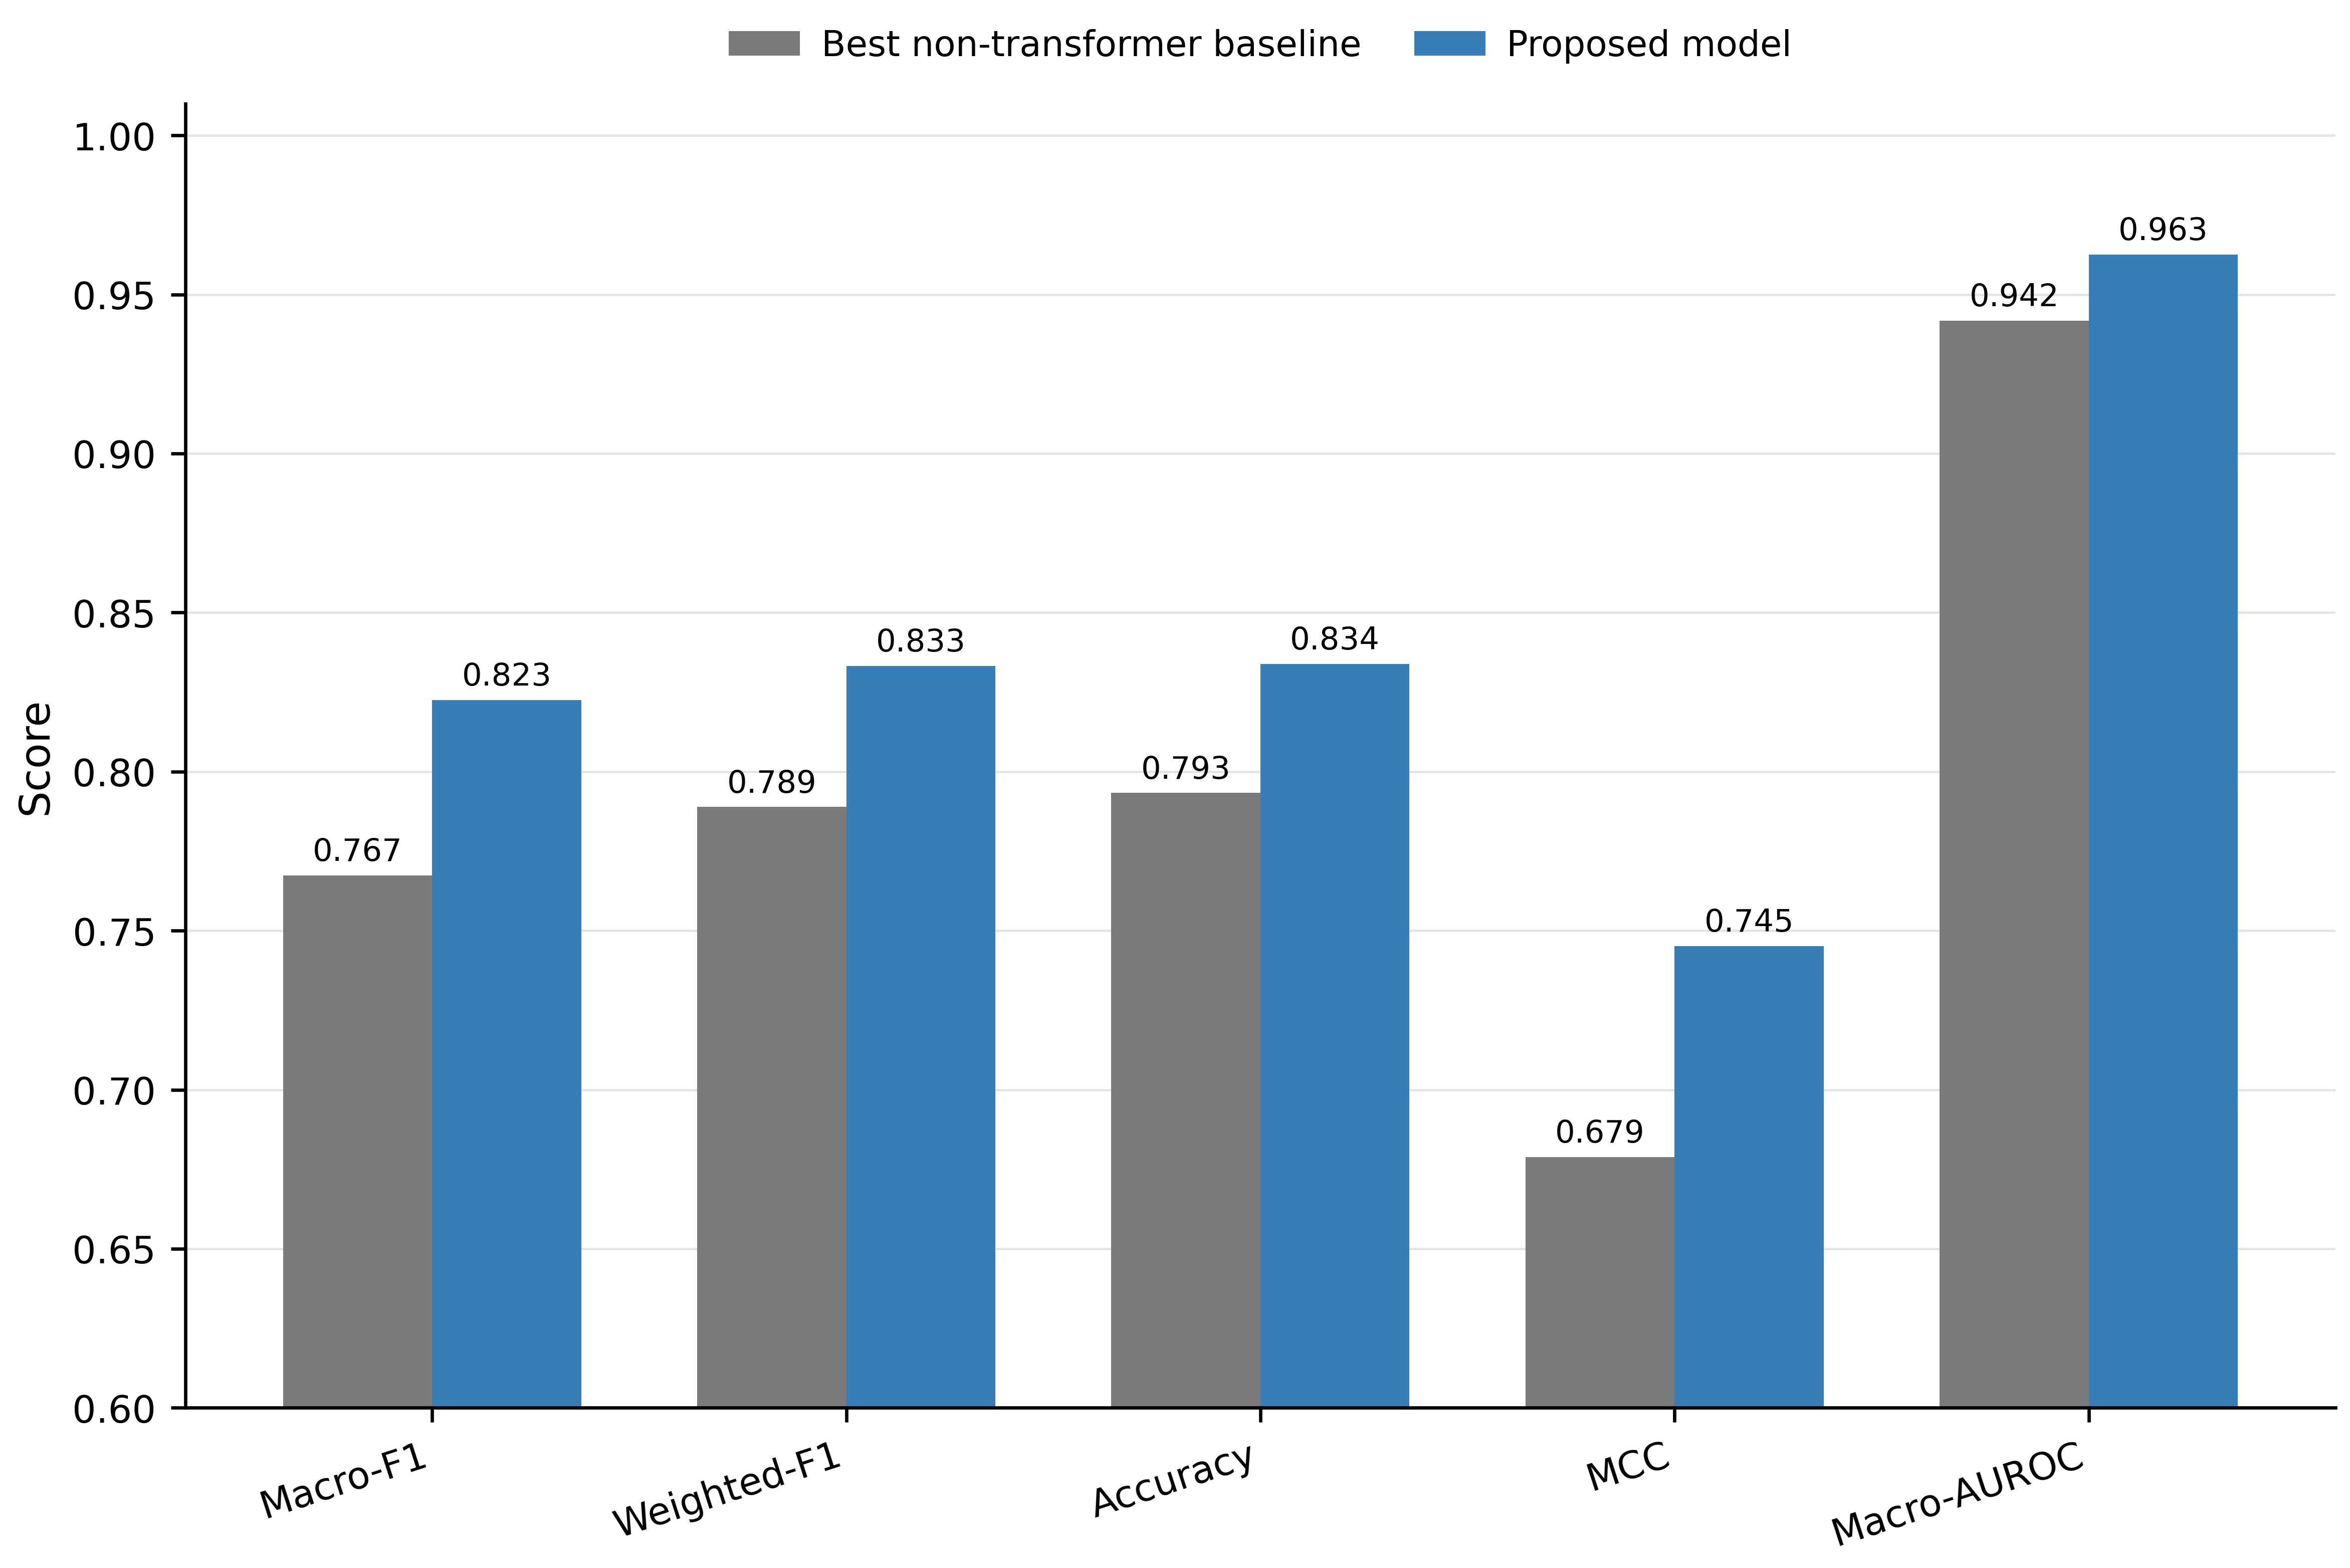
\includegraphics[width=\textwidth]{fig02_main_results.png}
\caption{Proposed model vs.\ strongest baseline.}
\label{fig:main}
\end{subfigure}\hfill
\begin{subfigure}{0.49\textwidth}
\centering
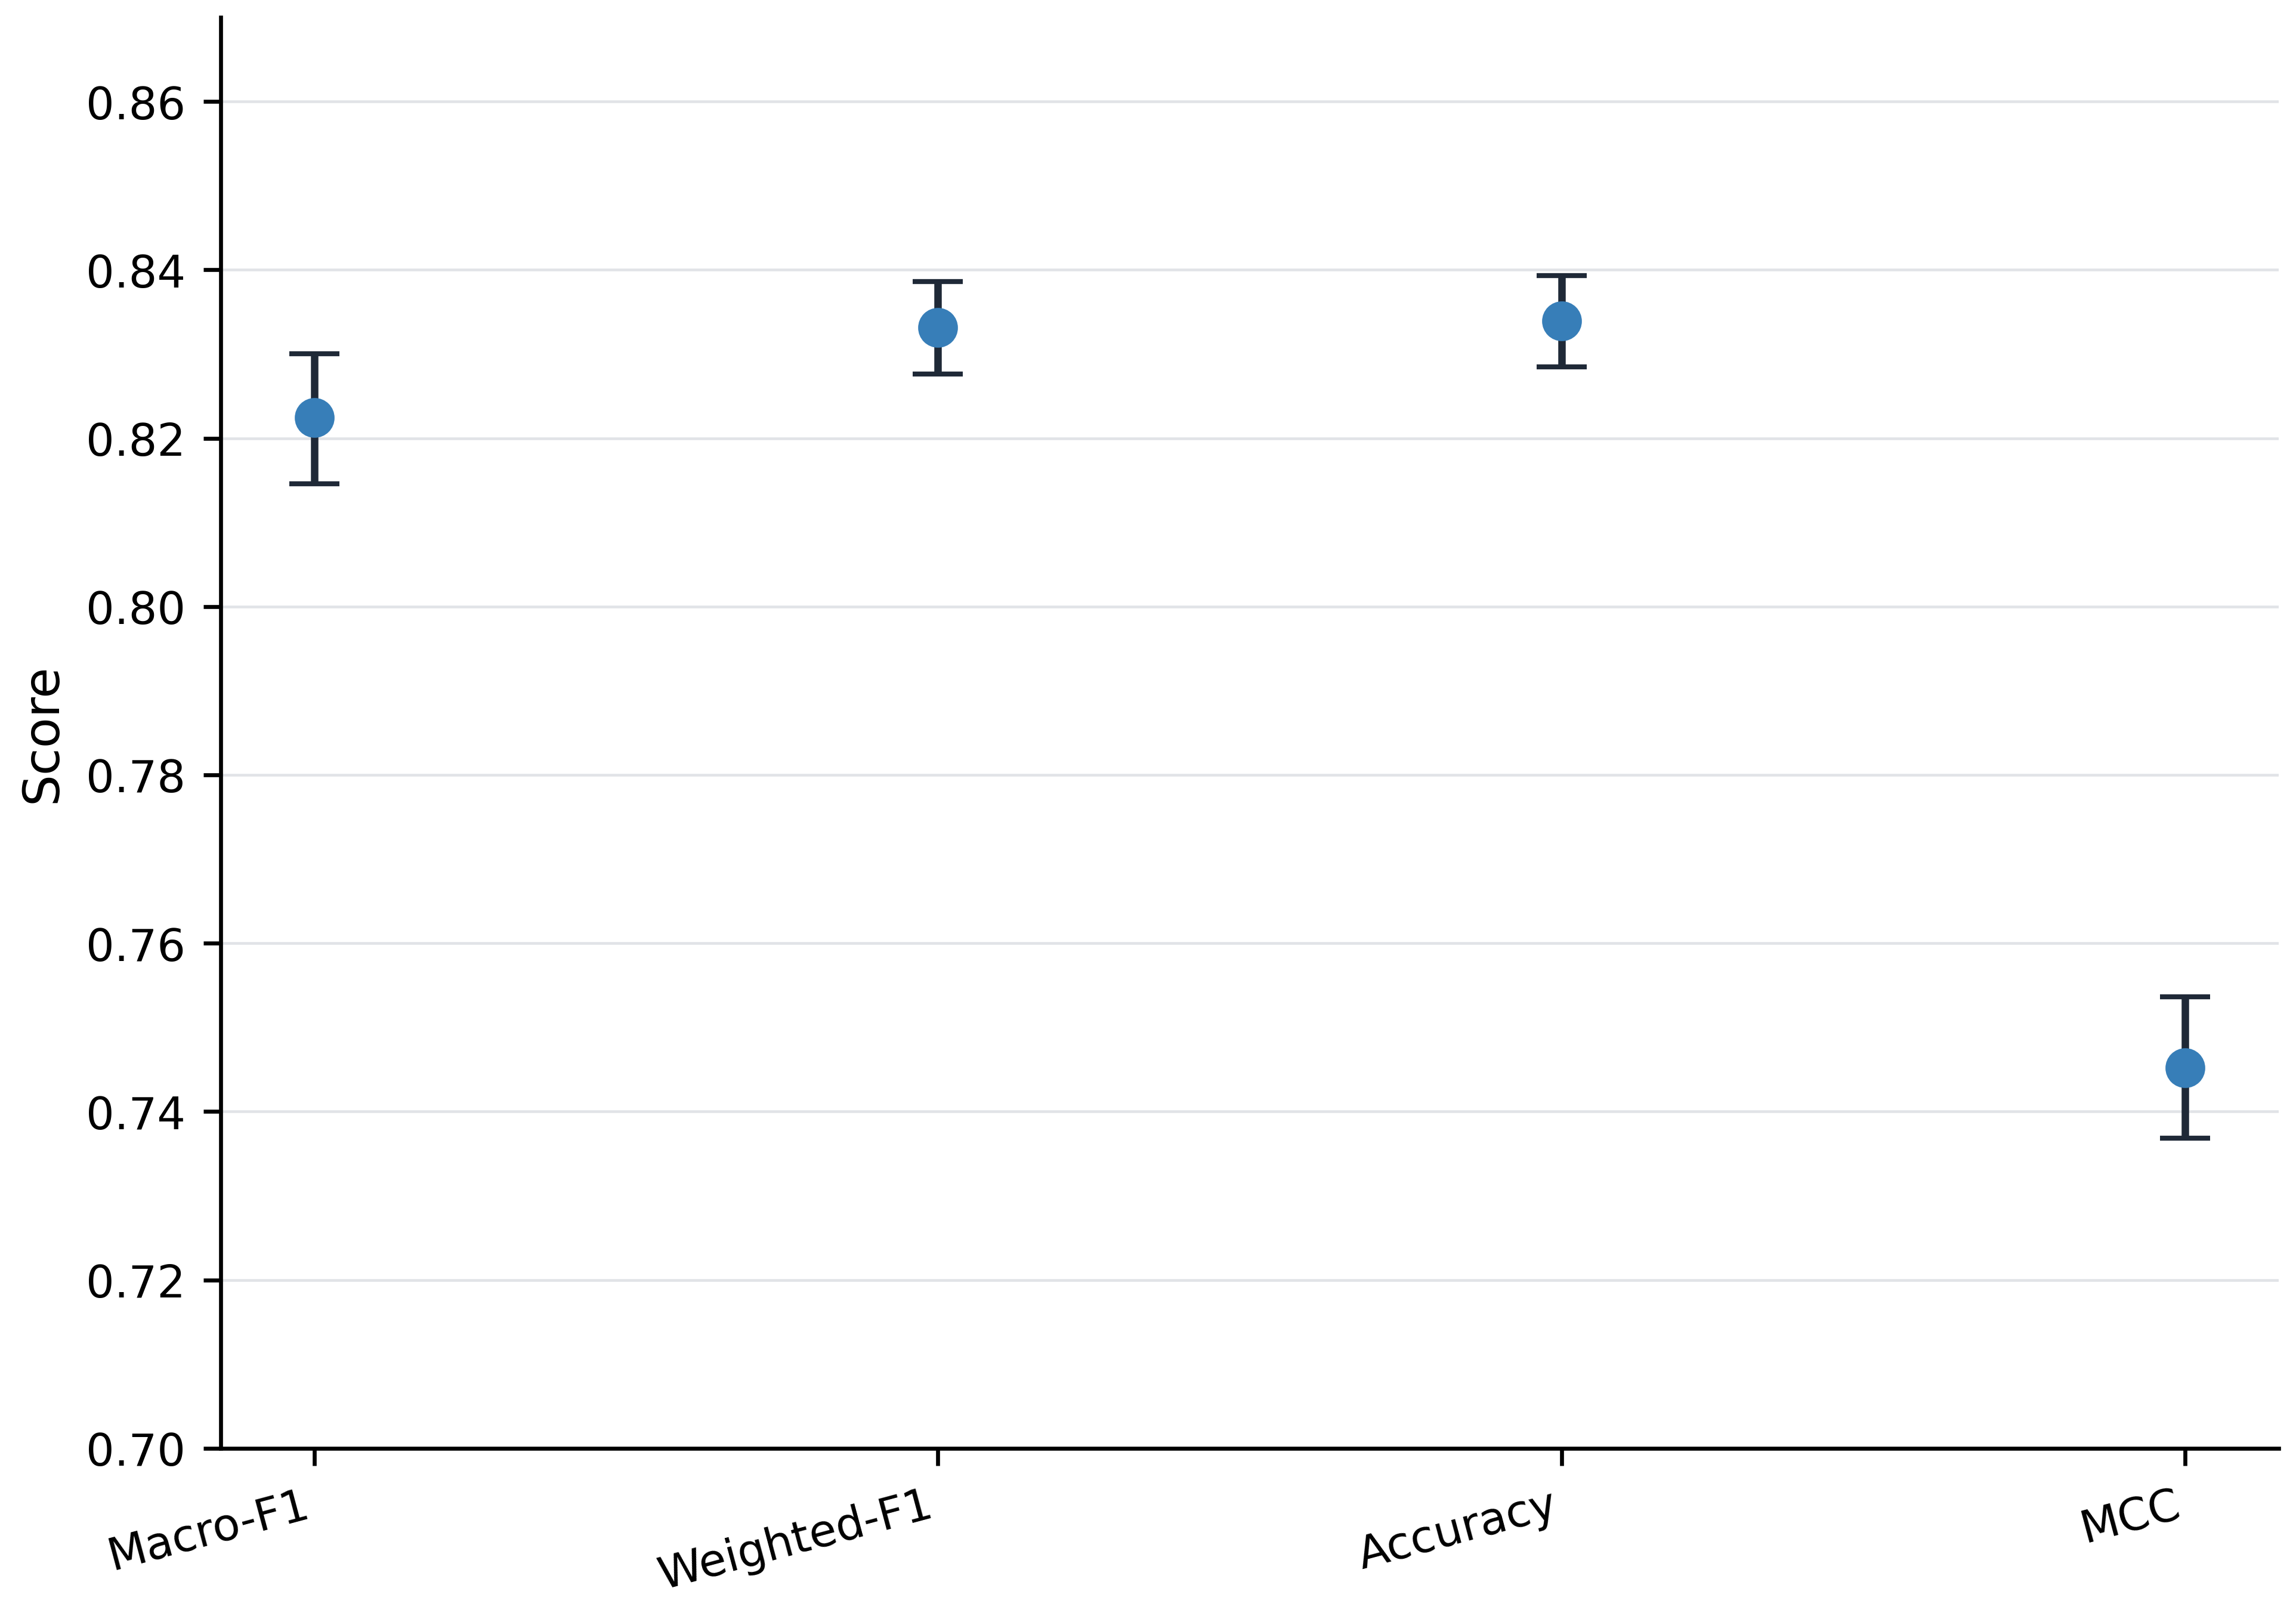
\includegraphics[width=\textwidth]{fig11_bootstrap_ci.png}
\caption{Headline metrics with bootstrap 95\% CIs.}
\label{fig:ci}
\end{subfigure}
\caption{In-domain test performance. The proposed model reports a higher point estimate than the strongest retained non-transformer baseline on every metric, and the bootstrap intervals are narrow (Macro-F1 width 0.0154).}
\label{fig:main-combined}
\end{figure}

Per-backbone single-run scores (\cref{tab:perrun}) also serve as the transformer baseline suite, since each row is a pretrained encoder fine-tuned with the identical configuration. The table spans two evaluation scopes and keeps them apart. BanglishBERT, MuRIL, and XLM-R are full-scope models scored on the complete test split, and their best single run is MuRIL at 0.8084, with BanglishBERT at 0.8083 and XLM-R at 0.8052 close behind. BanglaBERT is restricted to Bangla-script rows by the routing rule, so its 0.8154 is measured on the Bangla-script subset alone and cannot be lined up against the full-scope rows. The ensemble's Macro-F1 is 0.8225, compared with 0.8084 for the strongest retained full-scope member. This is an unpaired point-estimate difference, because the required paired member predictions were not retained for the final configuration. The result should not be described as statistically significant or as proof of complementary errors.

\begin{table}[!htbp]
\centering
\caption{Per-backbone, per-seed single-run scores, each trained with the identical configuration. BanglishBERT, MuRIL, and XLM-R are full-scope and are scored on the complete test split ($n = 18{,}865$). BanglaBERT is restricted to Bangla-script rows by the routing rule of \cref{sec:scriptaware}, so its rows are scored on the Bangla-script test subset only and are not directly comparable with the full-scope rows.}
\label{tab:perrun}
\small
\begin{tabular}{@{}llccccc@{}}
\toprule
\textbf{Backbone} & \textbf{Seed} & \textbf{Macro-F1} & \textbf{Weighted-F1} & \textbf{Accuracy} & \textbf{MCC} & \textbf{AUROC} \\
\midrule
BanglishBERT & 42 & 0.8069 & 0.8201 & 0.8206 & 0.7252 & 0.9567 \\
BanglishBERT & 123 & 0.7996 & 0.8124 & 0.8161 & 0.7151 & 0.9547 \\
BanglishBERT & 456 & 0.8083 & 0.8200 & 0.8213 & 0.7261 & 0.9568 \\
BanglaBERT$^{\dagger}$ & 42 & 0.8105 & 0.8178 & 0.8177 & 0.7545 & 0.9602 \\
BanglaBERT$^{\dagger}$ & 123 & 0.8154 & 0.8211 & 0.8218 & 0.7603 & 0.9599 \\
BanglaBERT$^{\dagger}$ & 456 & 0.8149 & 0.8205 & 0.8216 & 0.7600 & 0.9615 \\
MuRIL & 42 & 0.8055 & 0.8177 & 0.8185 & 0.7231 & 0.9521 \\
MuRIL & 123 & \textbf{0.8084} & 0.8216 & 0.8222 & \textbf{0.7284} & 0.9502 \\
MuRIL & 456 & 0.8066 & 0.8198 & 0.8210 & 0.7259 & 0.9523 \\
XLM-R & 42 & 0.8052 & 0.8159 & 0.8161 & 0.7199 & 0.9538 \\
XLM-R & 123 & 0.8016 & 0.8144 & 0.8145 & 0.7166 & 0.9503 \\
XLM-R & 456 & 0.8035 & 0.8173 & 0.8181 & 0.7215 & 0.9501 \\
\bottomrule
\end{tabular}

\vspace{2pt}
{\footnotesize $^{\dagger}$Bangla-script specialist: trained and evaluated on Bangla-script rows only, so these
scores are over the Bangla-script test subset and are not comparable with the full-scope rows above.
Bold marks the best full-scope run.}
\end{table}

\subsection{Zero-Shot LLM Reference}
\label{sec:llm-baseline}

We evaluate Gemini 2.5 Flash under one fixed zero-shot prompt \citep{google2025gemini25}. The prompt gave the same five-class definitions and priority rule the annotators used, and the model labelled each of the 18{,}865 test comments individually at temperature $0$ with an instruction to emit the bare label word. Replies were matched against the five class names, and a reply matching none of them fell back to \emph{none}, the majority class. It obtains a Macro-F1 of 0.5597 on the retained test split (\cref{tab:llm}). Because only one model and prompt were evaluated and aggregate parse-failure records were not retained, this result is a limited reference rather than a general comparison of prompted language models.

\begin{table}[!htbp]
\centering
\caption{Zero-shot large-language-model reference against the proposed supervised model on the in-domain test split ($n = 18{,}865$).}
\label{tab:llm}
\small
\begin{tabular}{@{}lcccc@{}}
\toprule
\textbf{System} & \textbf{Macro-F1} & \textbf{Weighted-F1} & \textbf{Accuracy} & \textbf{MCC} \\
\midrule
Gemini 2.5 Flash (zero-shot) & 0.5597 & 0.6684 & 0.6647 & 0.4957 \\
\textbf{Proposed model (supervised)} & \textbf{0.8225} & \textbf{0.8332} & \textbf{0.8339} & \textbf{0.7452} \\
\bottomrule
\end{tabular}
\end{table}

The supervised ensemble reports a higher point estimate than this single zero-shot configuration. Prompt design, model choice, and parsing behavior were not varied, so no broader conclusion about language-model-based moderation is supported.

\subsection{Per-Class Performance and Error Analysis}
\label{sec:perclass-results}

\Cref{tab:perclass} reports per-class performance on the in-domain test split. \emph{Religious} and \emph{none} obtain the highest F1 values, 0.9031 and 0.8771. \emph{Sexual} follows at 0.8238, and the two lowest are \emph{threat} at 0.7689 and \emph{abusive} at 0.7397. \emph{Threat} has the smallest support, 638 test items, and correspondingly the widest bootstrap interval, $[0.7424, 0.7949]$. \emph{Abusive} is the residual bucket, absorbing troll, personal, political, and spam content, so its boundary with \emph{none} is less sharply defined.

\begin{table}[!htbp]
\centering
\caption{Per-class precision, recall, F1, and bootstrap 95\% confidence interval on the in-domain test split. Support is the number of test comments in each class.}
\label{tab:perclass}
\small
\begin{tabular}{@{}lccccr@{}}
\toprule
\textbf{Class} & \textbf{Precision} & \textbf{Recall} & \textbf{F1} & \textbf{95\% CI (F1)} & \textbf{Support} \\
\midrule
Religious & 0.9221 & 0.8848 & 0.9031 & $[0.8921,\ 0.9137]$ & 1{,}606 \\
None & 0.8622 & 0.8925 & 0.8771 & $[0.8723,\ 0.8819]$ & 9{,}463 \\
Sexual & 0.8359 & 0.8120 & 0.8238 & $[0.8115,\ 0.8358]$ & 2{,}165 \\
Threat & 0.7878 & 0.7508 & 0.7689 & $[0.7424,\ 0.7949]$ & 638 \\
Abusive & 0.7532 & 0.7266 & 0.7397 & $[0.7297,\ 0.7497]$ & 4{,}993 \\
\midrule
\textbf{Macro avg.} & 0.8322 & 0.8133 & 0.8225 & $[0.8146,\ 0.8300]$ & 18{,}865 \\
\bottomrule
\end{tabular}
\end{table}

Every class has positive support in the overall test-split results. For script-stratified results, a class with zero gold support contributes an F1 of $0$ to the five-class mean. This applies to Romanized Bangla, whose consolidated gold set contains no \emph{threat} examples, so \cref{sec:scriptmask-results} reports both the fixed five-class value and a supported-class value and labels each explicitly.

The confusion matrix (\cref{fig:confusion}) shows where the errors concentrate. The largest off-diagonal mass is the \emph{abusive} and \emph{none} pair, with 1{,}081 true-\emph{abusive} comments predicted \emph{none} and 856 true-\emph{none} predicted \emph{abusive}. The next-largest confusions (\cref{fig:topconf}) are \emph{sexual} predicted as \emph{abusive} (225) and \emph{abusive} predicted as \emph{sexual} (195). \emph{Threat}, despite the smallest support, keeps 479 of its items on the diagonal. The three summarized confusion patterns account for 2{,}405 of the model's 3{,}133 errors, or 76.8\%.

\begin{figure}[!htbp]
\centering
\begin{subfigure}{0.52\textwidth}
\centering
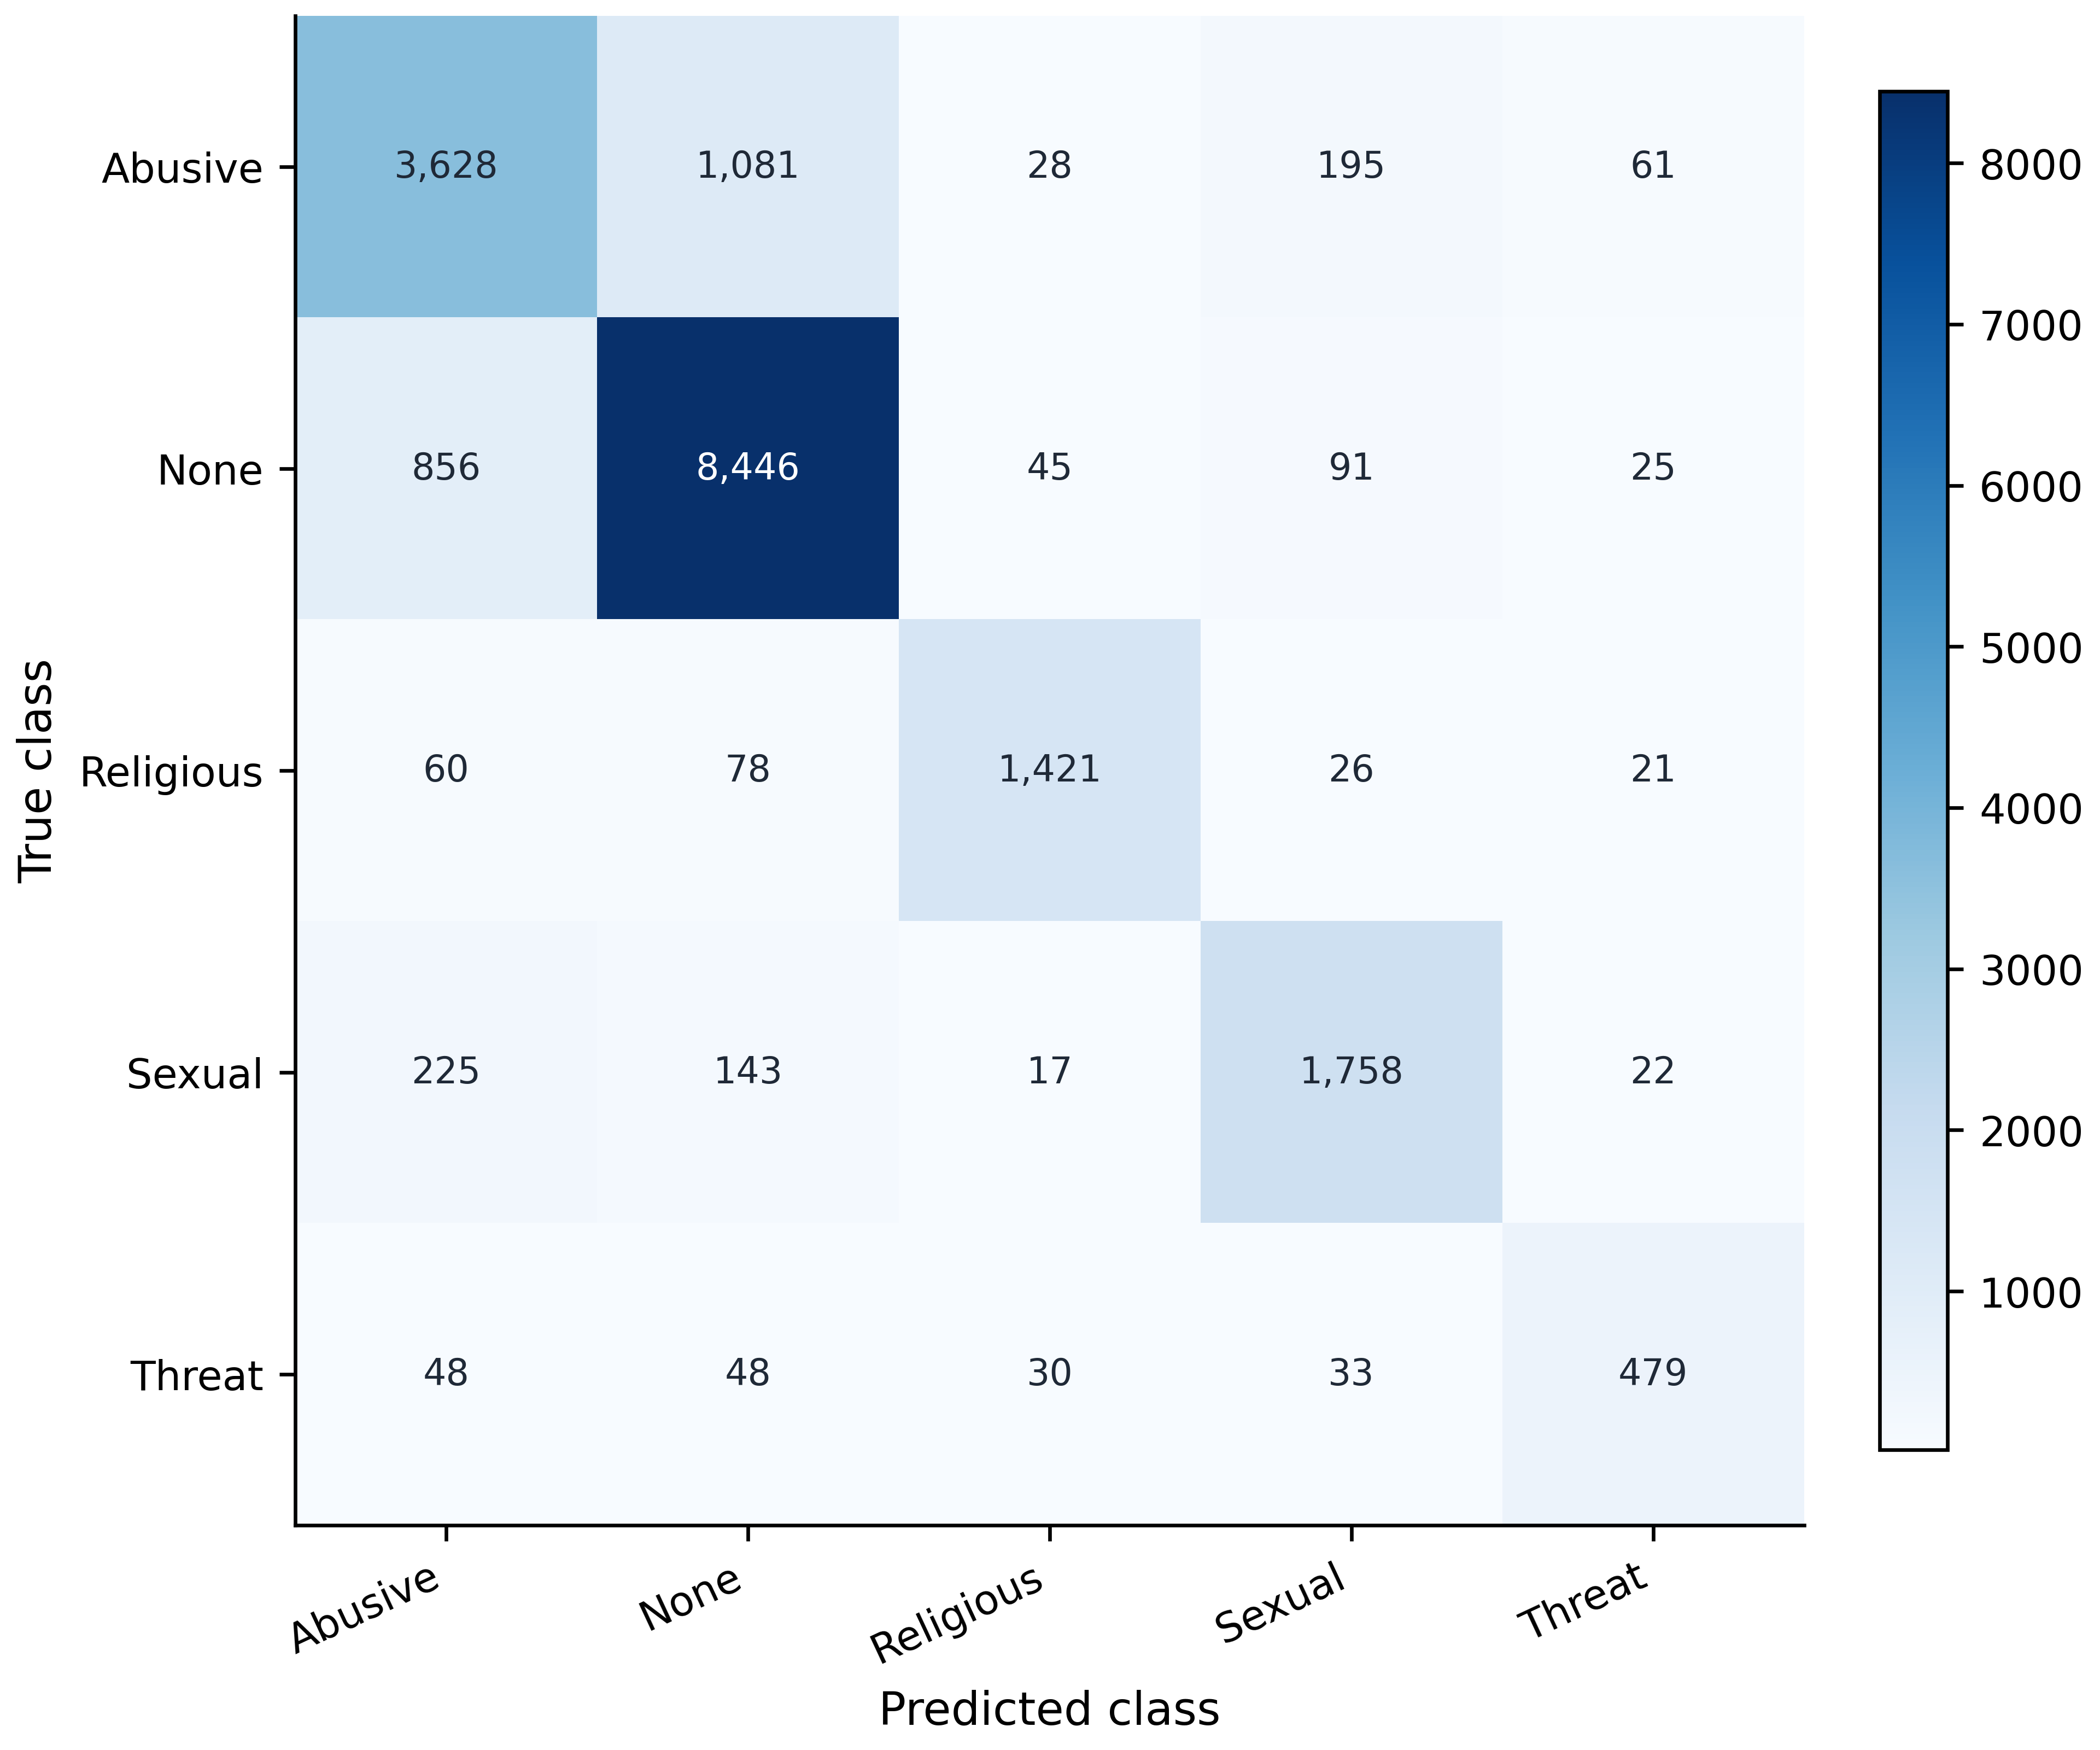
\includegraphics[width=\textwidth]{fig04_confusion_matrix.png}
\caption{Counts.}
\label{fig:confusion}
\end{subfigure}\hfill
\begin{subfigure}{0.46\textwidth}
\centering
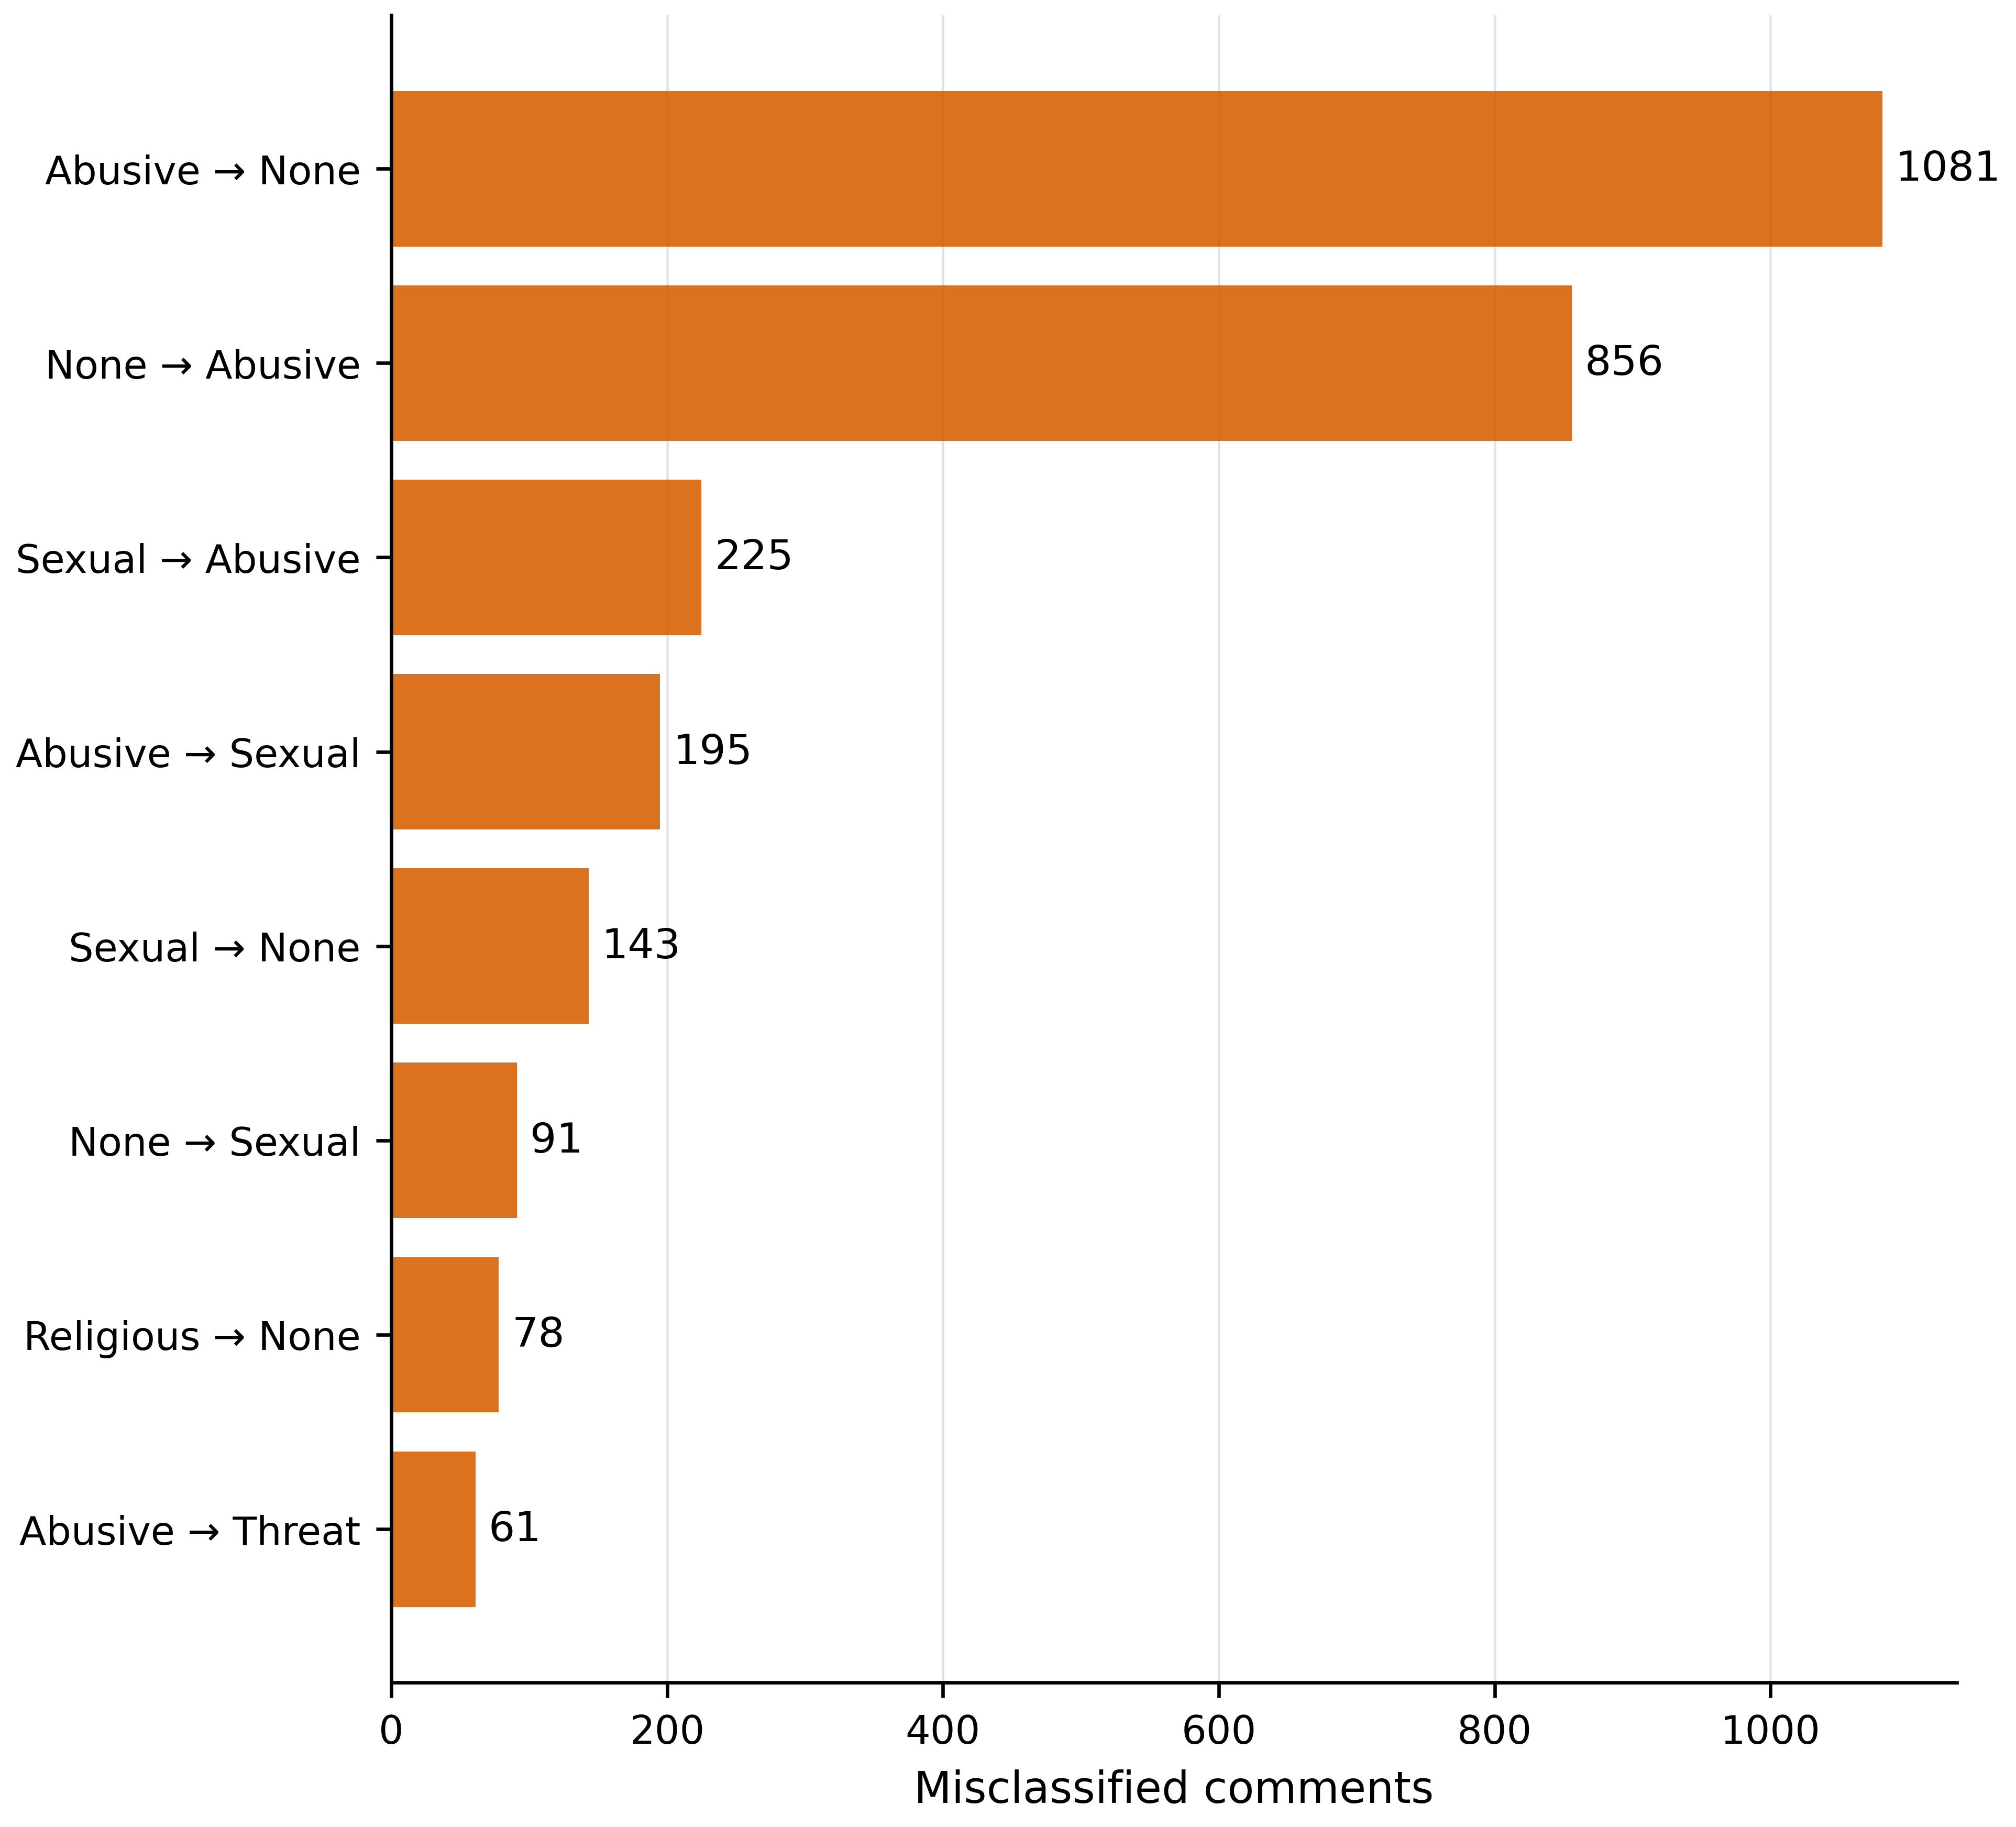
\includegraphics[width=\textwidth]{fig05_top_confusions.png}
\caption{Largest off-diagonal error pairs.}
\label{fig:topconf}
\end{subfigure}
\caption{Confusion structure of the proposed model on the in-domain test split. The largest off-diagonal counts occur between Abusive and None.}
\label{fig:confusion-combined}
\end{figure}

Most errors occur between Abusive and None and between Sexual and Abusive (\cref{tab:errorpatterns}). These patterns may reflect semantic overlap or differences in annotation policy between the four source teams, but the present study does not include a coded qualitative error analysis. The explanations are therefore hypotheses rather than demonstrated causes. A third pattern, \emph{threat} predicted as \emph{abusive}, is consistent with \emph{threat} recall (0.7508) trailing its precision (0.7878), though a confusion matrix alone cannot establish the mechanism.

\begin{table}[!htbp]
\centering
\caption{The three largest off-diagonal error patterns, with a hypothesised mechanism and the number of test comments each accounts for. Together they cover 2{,}405 of the 3{,}133 errors.}
\label{tab:errorpatterns}
\small
\begin{tabularx}{\textwidth}{@{}l>{\raggedright\arraybackslash}Xr@{}}
\toprule
\textbf{Error pattern} & \textbf{Mechanism} & \textbf{Count} \\
\midrule
Abusive $\leftrightarrow$ None & Intent ambiguity: sarcasm, in-group language, and blunt-but-clean criticism are not separable from the surface text alone. & 1{,}937 \\
Sexual $\leftrightarrow$ Abusive & Content overlap: misogynistic comments are also generically abusive, and the single-label scheme forces one class. & 420 \\
Threat $\to$ Abusive & Minority dilution: implicit threats without violent keywords drift into the larger \emph{abusive} bucket. & 48 \\
\bottomrule
\end{tabularx}
\end{table}

\subsection{Ablations}
\label{sec:ablation-results}

\paragraph{Component sensitivity.} \Cref{tab:component} starts from plain cross-entropy and adds components one at a time, with three seeds per configuration. In this fixed BanglishBERT sensitivity configuration, adding FGM increases Macro-F1 from $0.7961$ to $0.8071$, a difference of $0.0110$ that is larger than the observed seed spread of the reference ($0.0022$). We state only that FGM increases Macro-F1 by 0.0110 over cross-entropy in this configuration, not that it is universally decisive.

The remaining rows measure each additional component against cross-entropy with FGM. EMA is 0.0022 higher and R-Drop 0.0012 higher, multi-sample dropout is 0.0003 lower, and focal loss with class weighting, the balanced sampler, and the full stack are 0.0016, 0.0076, and 0.0029 lower. Because the configurations differ and each uses only three seeds, we attach no significance claims to these differences. Cross-entropy with FGM was retained as the transparent and computationally modest choice. The sensitivity configuration also differs from the main training configuration in batch size, learning rates, and epoch budget, so these values are not a tuned leaderboard. \Cref{fig:ablation} plots the same measurements.

\begin{table}[!htbp]
\centering
\caption{Component sensitivity on the retained test split using BanglishBERT and three seeds per configuration (mean $\pm$ std). CE is the initial reference. FGM is then added, and each subsequent row adds the named component to CE$+$FGM. Differences are descriptive rather than significance tests.}
\label{tab:component}
\small
\begin{tabular}{@{}lcccccr@{}}
\toprule
\textbf{Configuration} & \textbf{Macro-F1} & \textbf{Weighted-F1} & \textbf{Accuracy} & \textbf{MCC} & \textbf{AUROC} & \textbf{$\Delta_{\mathrm{CE+FGM}}$} \\
\midrule
CE only (initial reference) & $0.7961 \pm 0.0022$ & 0.8087 & 0.8093 & 0.7079 & 0.9470 & NA \\
CE $+$ FGM (reference) & $0.8071 \pm 0.0009$ & 0.8199 & 0.8218 & 0.7262 & 0.9557 & $0.0000$ \\
CE $+$ FGM $+$ focal $+$ class weights & $0.8055 \pm 0.0012$ & 0.8178 & 0.8197 & 0.7232 & 0.9553 & $-0.0016$ \\
CE $+$ FGM $+$ balanced sampler & $0.7995 \pm 0.0026$ & 0.8115 & 0.8114 & 0.7129 & 0.9428 & $-0.0076$ \\
CE $+$ FGM $+$ multi-sample dropout & $0.8068 \pm 0.0014$ & 0.8187 & 0.8207 & 0.7248 & 0.9564 & $-0.0003$ \\
CE $+$ FGM $+$ R-Drop & $0.8083 \pm 0.0006$ & 0.8206 & 0.8231 & 0.7280 & 0.9568 & $+0.0012$ \\
CE $+$ FGM $+$ EMA & $\mathbf{0.8093 \pm 0.0004}$ & 0.8212 & 0.8220 & 0.7273 & 0.9576 & $+0.0022$ \\
Full stack (all on) & $0.8042 \pm 0.0019$ & 0.8145 & 0.8143 & 0.7176 & 0.9529 & $-0.0029$ \\
\bottomrule
\end{tabular}
\end{table}

\begin{figure}[!htbp]
\centering
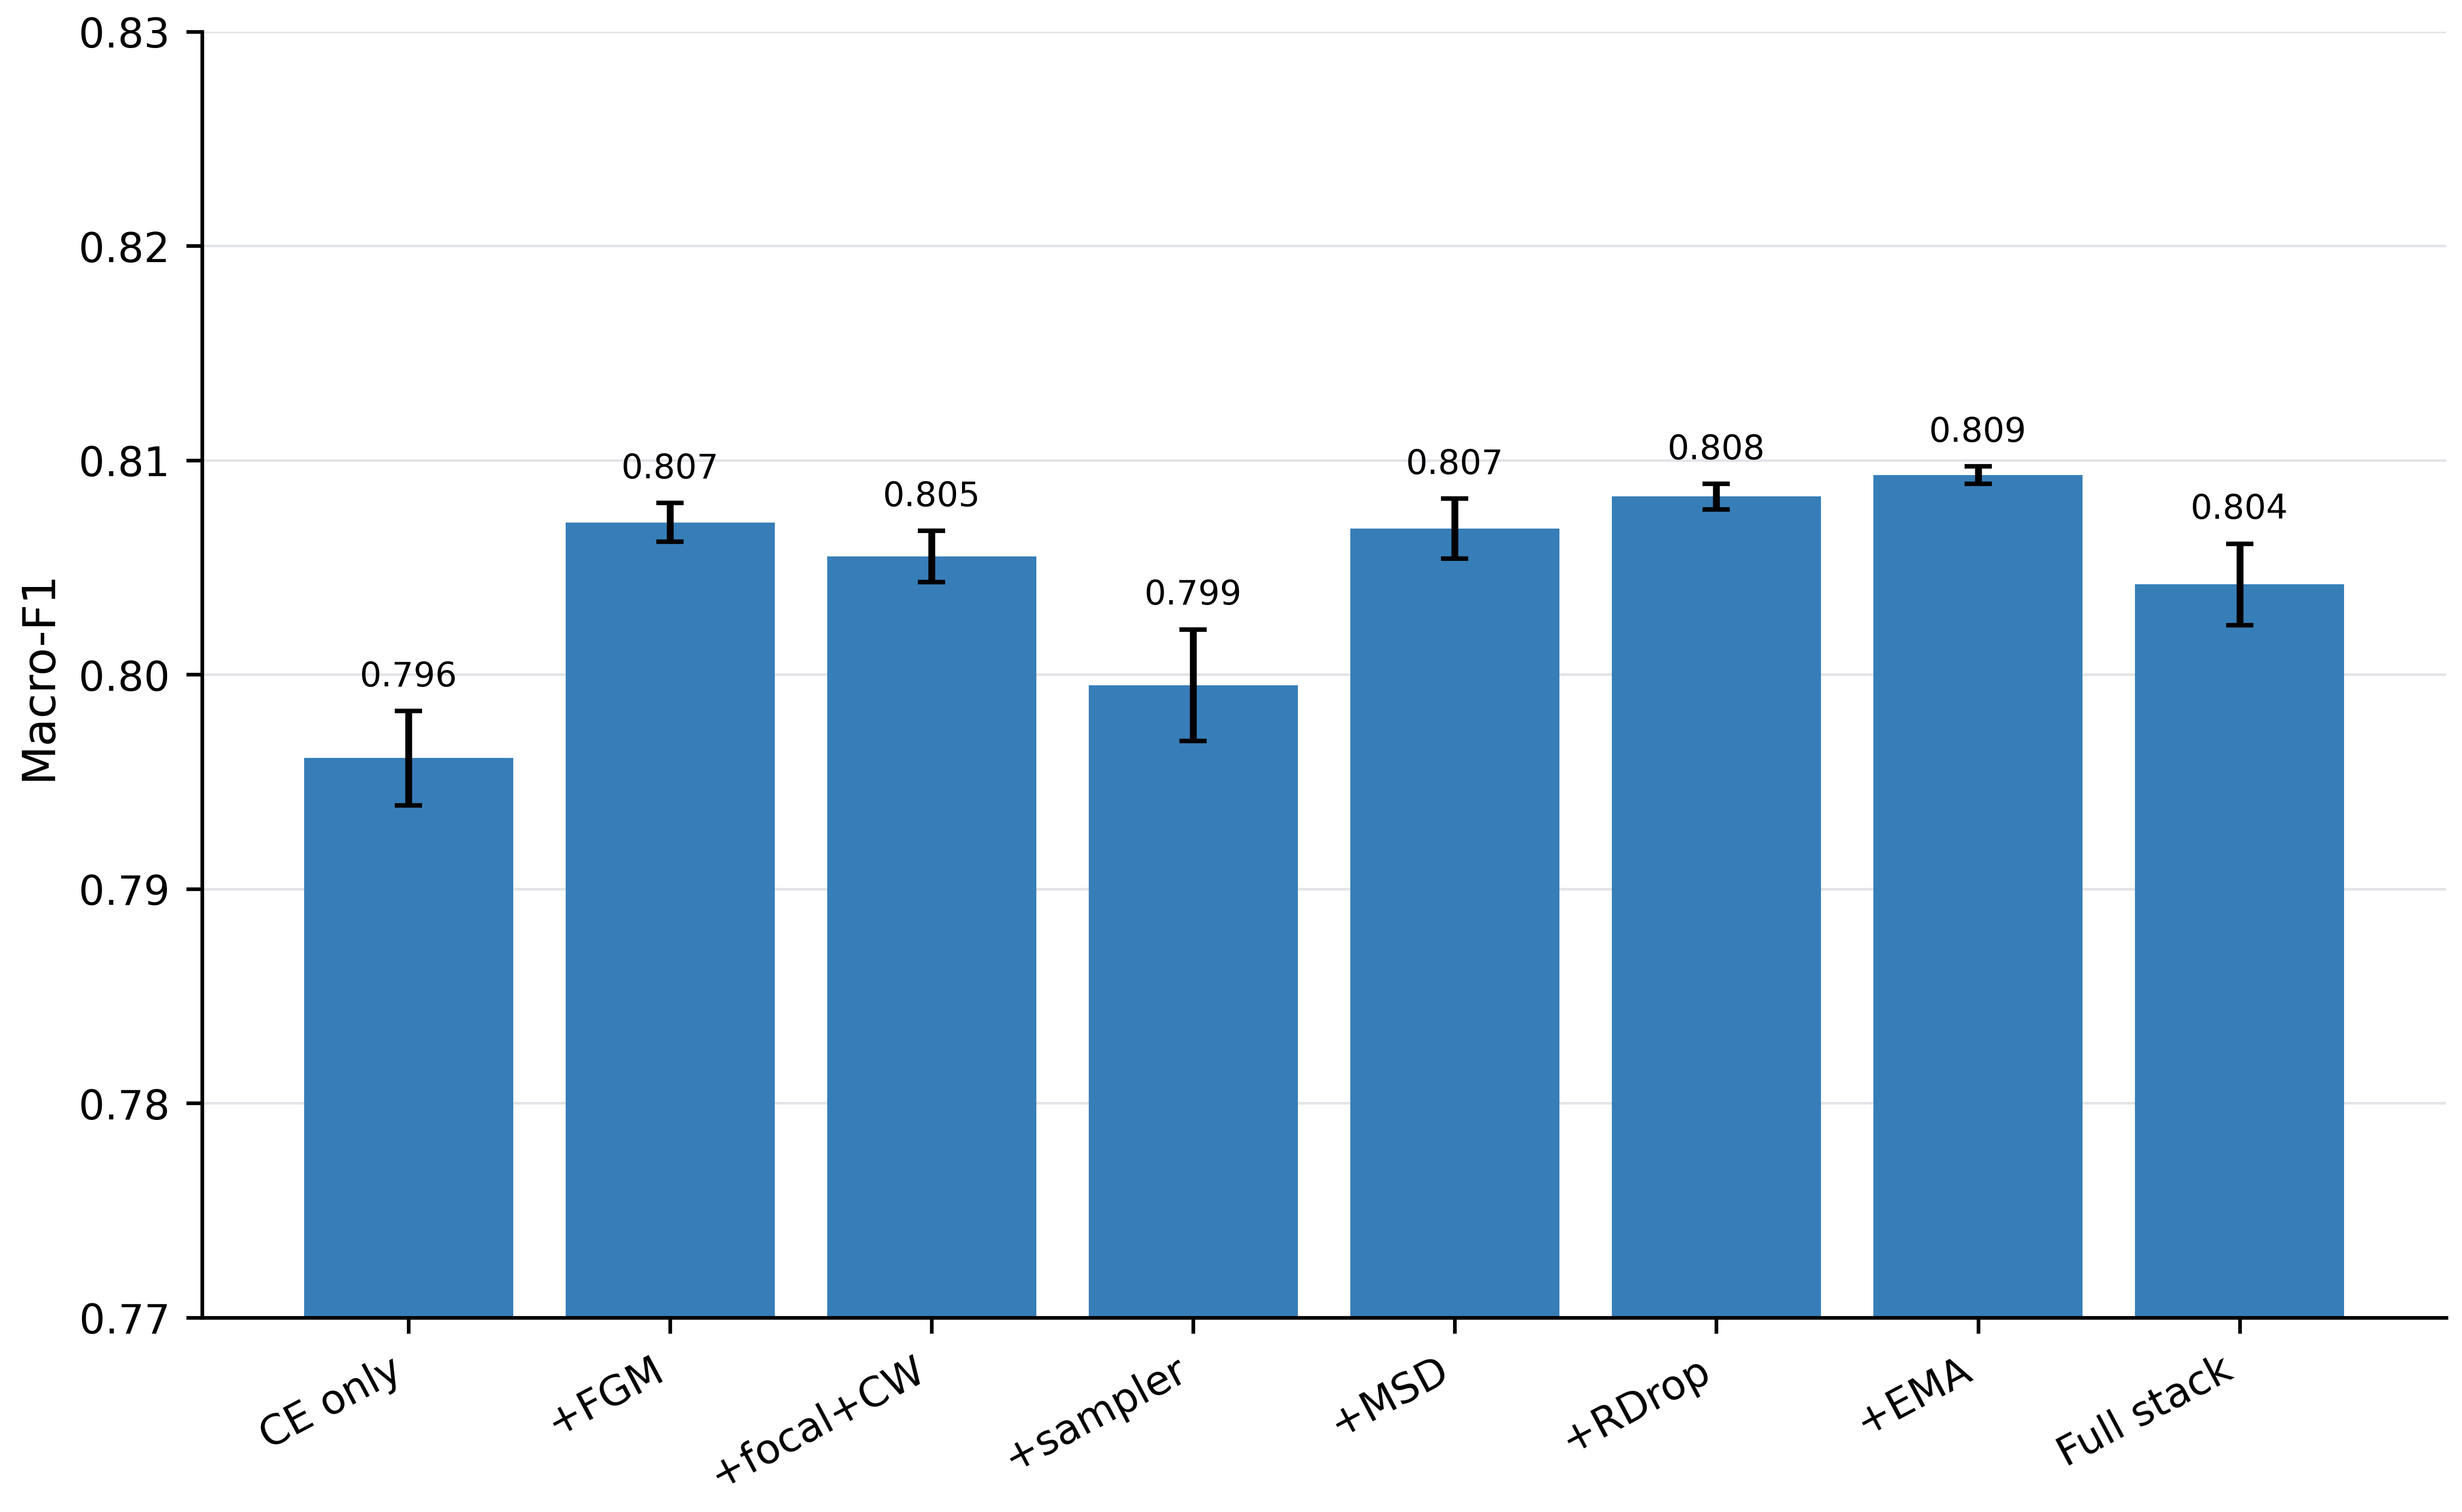
\includegraphics[width=0.82\textwidth]{fig06_component_ablation.png}
\caption{Component sensitivity, mean $\pm$ std over three seeds. FGM produces the largest first increase in this configuration, and the proposed model fine-tunes each backbone with cross-entropy and FGM.}
\label{fig:ablation}
\end{figure}

\paragraph{Taxonomy sensitivity.} The nine-class sensitivity configuration, which adds \texttt{personal}, \texttt{political}, \texttt{gender}, and \texttt{other}, produces a lower Macro-F1 than the five-class configuration, 0.6140 against 0.8073 (\cref{tab:taxonomy}, \cref{fig:taxonomy}). Weighted-F1 changes less because the majority classes dominate it. The result is consistent with limited support for several fine-grained classes, but the retained analysis does not establish support as the sole cause.

\begin{table}[!htbp]
\centering
\caption{Taxonomy sensitivity under the reported training configuration. The nine-class scheme has a substantially lower Macro-F1, while Weighted-F1 changes less.}
\label{tab:taxonomy}
\small
\begin{tabular}{@{}lccccc@{}}
\toprule
\textbf{Taxonomy} & \textbf{Macro-F1} & \textbf{Weighted-F1} & \textbf{Accuracy} & \textbf{MCC} & \textbf{AUROC} \\
\midrule
5-class (headline) & \textbf{0.8073} & 0.8203 & 0.8214 & 0.7255 & 0.9556 \\
9-class (ablation) & 0.6140 & 0.8020 & 0.8069 & 0.7071 & 0.9460 \\
\bottomrule
\end{tabular}
\end{table}

\begin{figure}[!htbp]
\centering
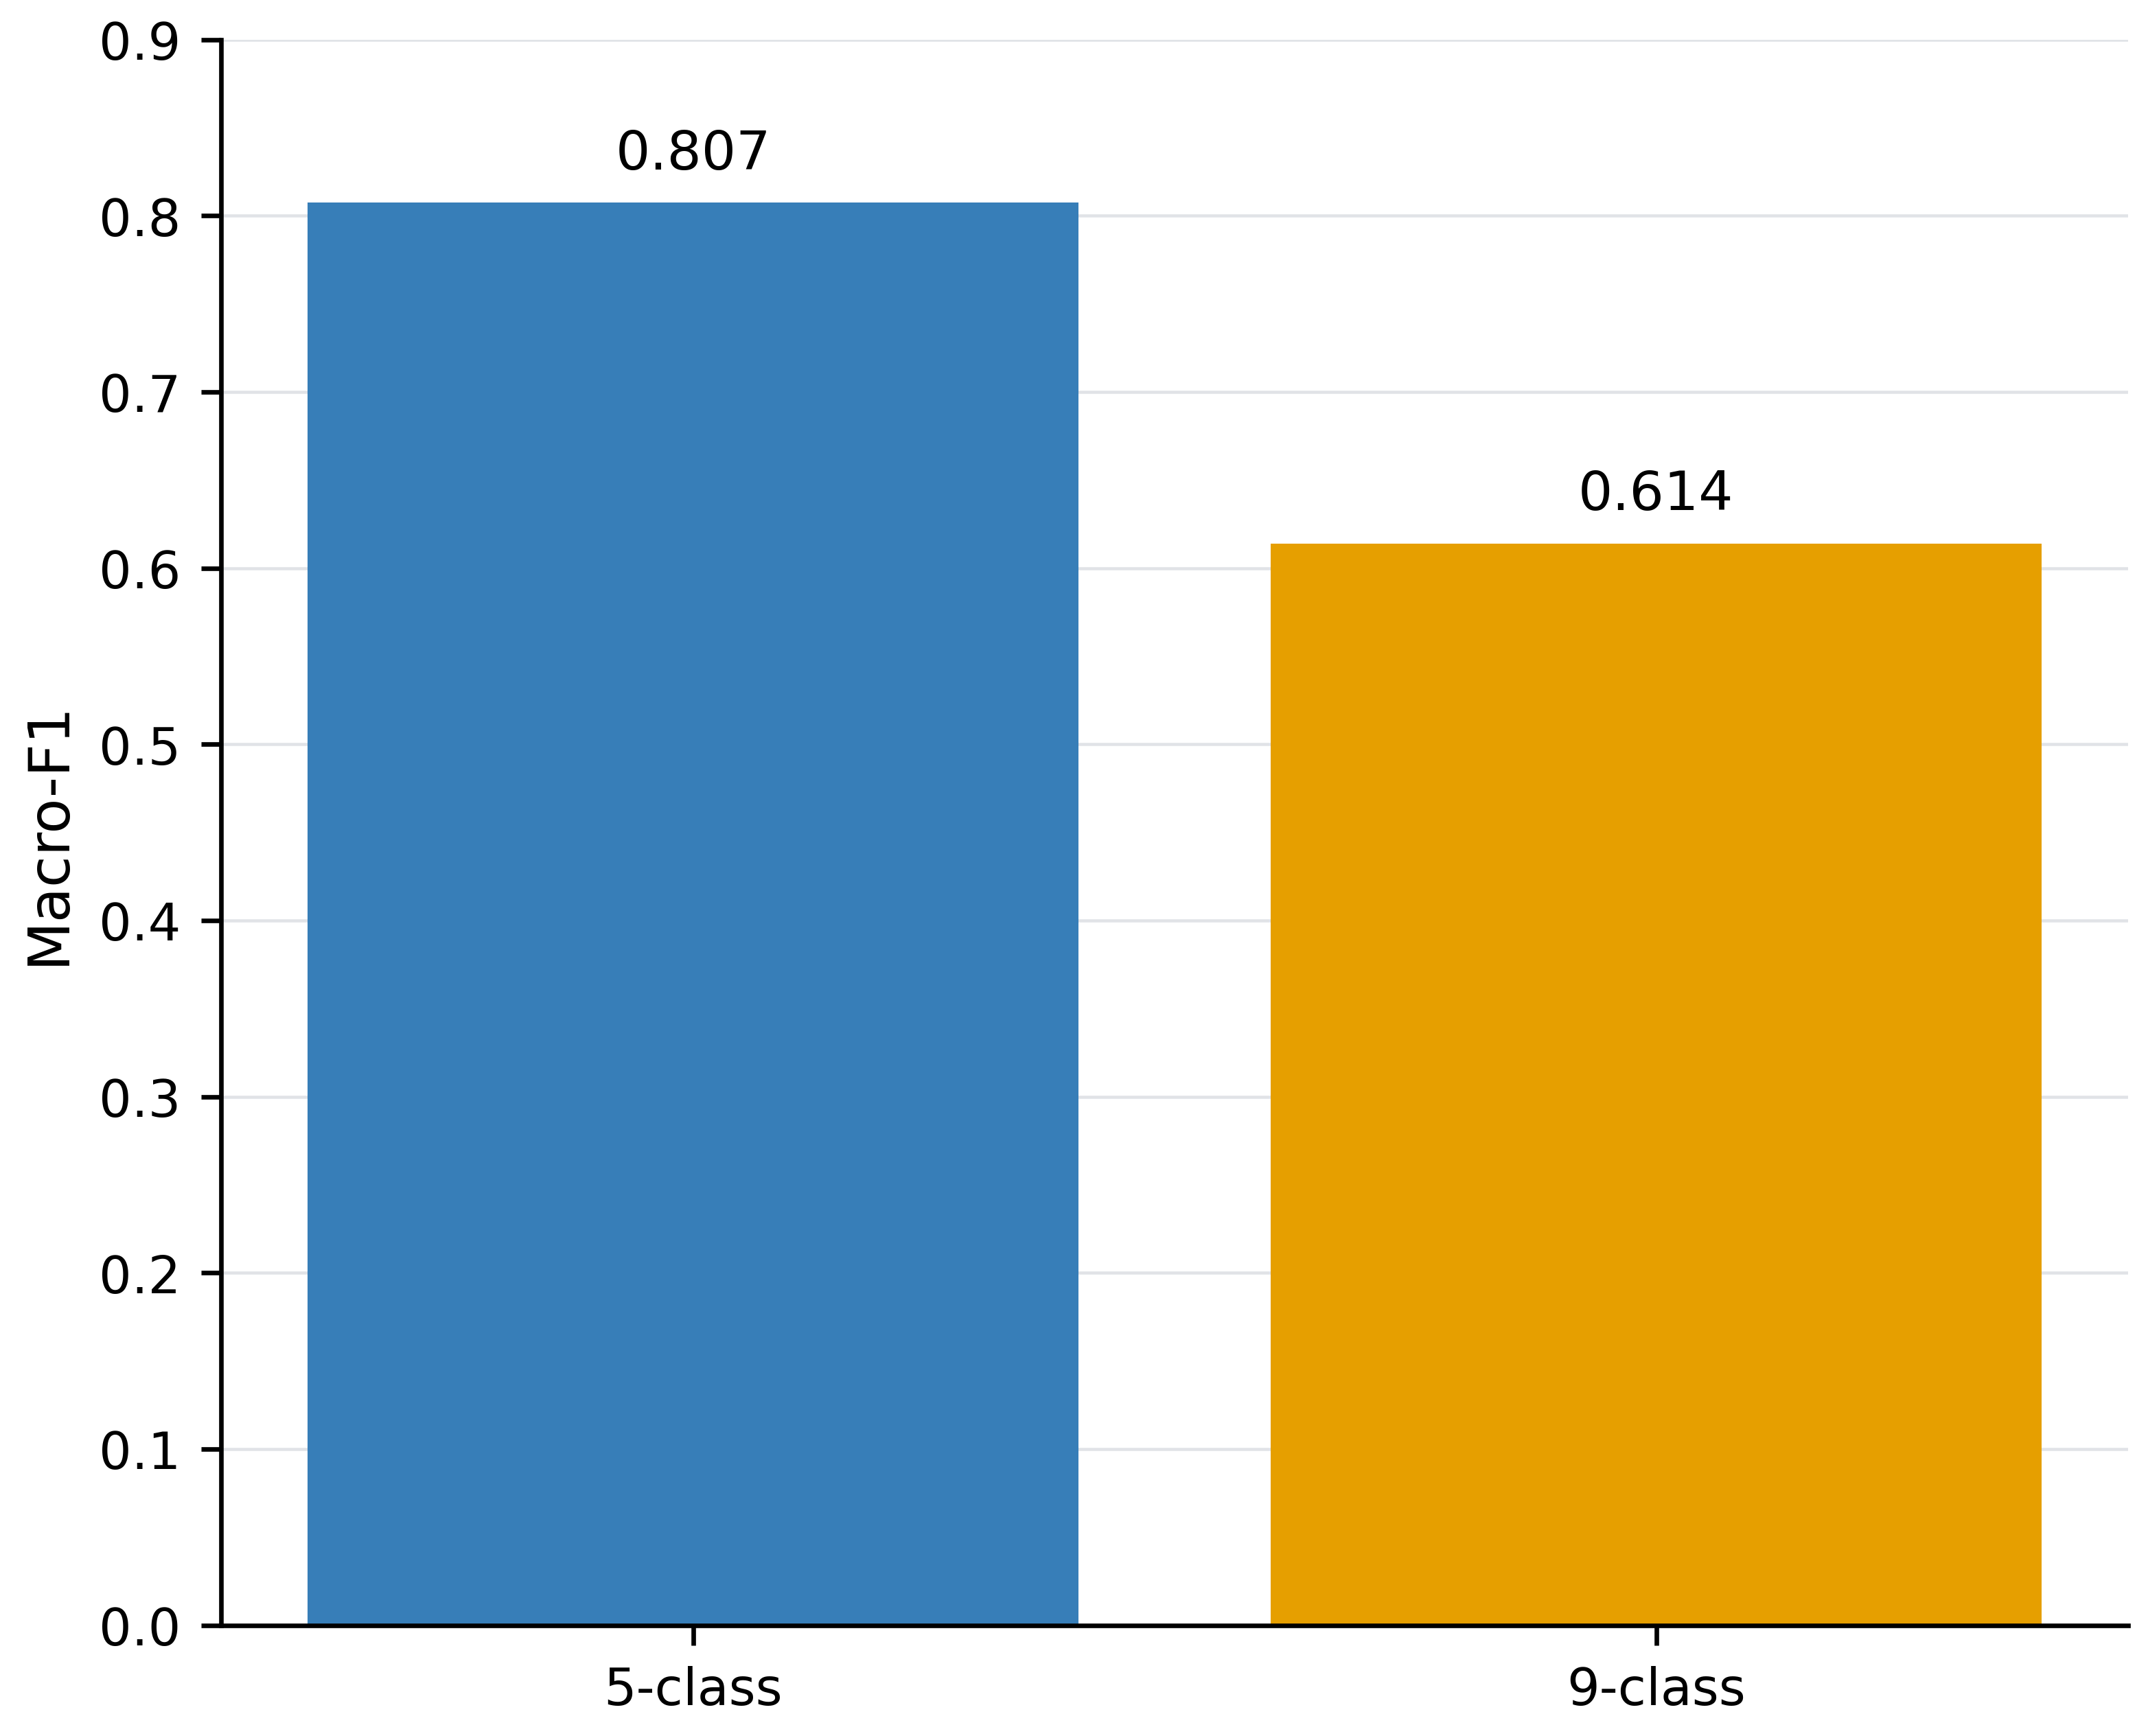
\includegraphics[width=0.52\textwidth]{fig07_taxonomy_ablation.png}
\caption{Taxonomy sensitivity. Macro-F1 is 0.6140 for the nine-class configuration and 0.8073 for the five-class configuration.}
\label{fig:taxonomy}
\end{figure}

\subsection{Script-Stratified Performance and Routing Sensitivity}
\label{sec:scriptmask-results}

\Cref{tab:script-results} reports final-ensemble performance by script on the in-domain test split. Romanized performance is reported under both the fixed five-class definition and a supported-class definition. The latter excludes classes with zero gold support in that subset.

\begin{table}[!htbp]
\centering
\caption{Final-ensemble results by script on the in-domain test split.}
\label{tab:script-results}
\small
\begin{tabular}{@{}lrrrrrr@{}}
\toprule
\textbf{Subset} & \textbf{$n$} & \textbf{Macro-F1$_5$} & \textbf{Macro-F1$_{\mathrm{sup}}$} & \textbf{Weighted-F1} & \textbf{Accuracy} & \textbf{MCC} \\
\midrule
All & 18{,}865 & 0.8225 & 0.8225 & 0.8332 & 0.8339 & 0.7452 \\
Bangla & 11{,}406 & 0.8303 & 0.8303 & 0.8368 & 0.8369 & 0.7805 \\
Romanized & 7{,}459 & 0.3900 & 0.4875 & 0.8238 & 0.8293 & 0.5771 \\
\bottomrule
\end{tabular}
\end{table}

The difference between the two Romanized Macro-F1 definitions is caused by zero \emph{threat} support. Religious and Sexual support is also small in the Romanized test subset, so their class-specific estimates are unstable. \Cref{tab:script-perclass} gives the per-class values behind these aggregates.

\begin{table}[!htbp]
\centering
\caption{Per-class F1 and support by script on the in-domain test split. Support counts are for the test partition, not the full benchmark.}
\label{tab:script-perclass}
\small
\begin{tabular}{@{}lrrrr@{}}
\toprule
\textbf{Class} & \textbf{Bangla F1} & \textbf{Bangla $n$} & \textbf{Romanized F1} & \textbf{Romanized $n$} \\
\midrule
Abusive & 0.7727 & 2{,}916 & 0.6917 & 2{,}077 \\
None & 0.8656 & 4{,}162 & 0.8861 & 5{,}301 \\
Religious & 0.9104 & 1{,}576 & 0.3721 & 30 \\
Sexual & 0.8340 & 2{,}114 & 0.0000 & 51 \\
Threat & 0.7689 & 638 & NA & 0 \\
\bottomrule
\end{tabular}
\end{table}

Because Romanized gold has zero support for \emph{threat}, and that class contributes zero to the five-class mean, the five-class Romanized Macro-F1 is capped at $4/5 = 0.80$ even for a classifier that is perfect on the four supported classes. Every Romanized five-class value must be read against that ceiling. The supported-class mean is a separate descriptive quantity and should not be conflated with the fixed five-class value. \Cref{tab:calibration} in \cref{sec:appendix} reports supported-class Macro-AUROC, expected calibration error, and Brier score for the same three subsets. Those are in-domain values and are not source-held-out calibration estimates.

\paragraph{Routing sensitivity.} The routing comparison in \cref{tab:scriptmask} uses a separate cached sensitivity configuration

\begin{table}[!htbp]
\centering
\caption{Routing sensitivity on the cached sensitivity configuration. Excluding BanglaBERT from Romanized comments is compared against letting every backbone vote on every comment. A zero-support class contributes an F1 of $0$ to the five-class mean.}
\label{tab:scriptmask}
\small
\begin{tabular}{@{}lcc@{}}
\toprule
\textbf{Setting} & \textbf{Romanized Macro-F1$_5$} & \textbf{Overall Macro-F1} \\
\midrule
No routing mask (all backbones vote) & 0.4568 & 0.8183 \\
Script-aware routing (proposed) & 0.4774 & 0.8176 \\
\bottomrule
\end{tabular}
\end{table}

In the sensitivity configuration, masking BanglaBERT changes Romanized five-class Macro-F1 from 0.4568 to 0.4774 and changes overall Macro-F1 from 0.8183 to 0.8176. These point estimates come from the sensitivity run, not the final ensemble. The routing mask is retained as a pretraining-scope constraint, but the available outputs do not establish a statistically significant improvement.

\paragraph{Fusion rule.} Uniform and validation-optimized fusion obtain Macro-F1 values of 0.8196 and 0.8193 in the same sensitivity configuration, against 0.8073 for the best single backbone in that study (\cref{tab:fusion}). Their 0.0003 difference does not support a claim that optimized weighting improves performance.

\begin{table}[!htbp]
\centering
\caption{Fusion-rule sensitivity on the cached sensitivity-run outputs. Uniform averaging and the validation-selected Nelder--Mead rule differ by 0.0003 Macro-F1.}
\label{tab:fusion}
\small
\begin{tabular}{@{}lc@{}}
\toprule
\textbf{Fusion rule} & \textbf{Macro-F1} \\
\midrule
Best single backbone & 0.8073 \\
Uniform average (equal weights) & 0.8196 \\
Nelder--Mead weighted (validation-selected) & 0.8193 \\
\bottomrule
\end{tabular}
\end{table}


\subsection{Cross-Source Robustness}
\label{sec:robustness-results}

Random-split evaluation measures generalisation to unseen comments from the same mixture. The source-held-out protocol of \cref{sec:splits} measures generalisation to an unseen source. Each of the three Bangla-script sources is held out in turn as the complete test set, the other two are split into training and validation, and the identifier-intersection assertion confirms that no comment appears in two partitions. BanTH is excluded because it supplies the benchmark's Romanized data, so holding it out would confound source and script shift. \Cref{tab:robustness} reports the three configurations with their split sizes, and \cref{fig:robustness} plots them against the in-domain value.

\begin{table}[!htbp]
\centering
\caption{Source-held-out results and split sizes for the three Bangla-script sources. Macro-F1 is the mean $\pm$ standard deviation over three seeds. The in-domain reference is a Macro-F1 of 0.8225.}
\label{tab:robustness}
\small
\begin{tabular}{@{}lrrrrr@{}}
\toprule
\textbf{Held-out source} & \textbf{$n_{\mathrm{train}}$} & \textbf{$n_{\mathrm{val}}$} & \textbf{$n_{\mathrm{test}}$} & \textbf{Macro-F1} & \textbf{MCC} \\
\midrule
Facebook-44K & 12{,}172 & 1{,}739 & 43{,}078 & $0.5850 \pm 0.0075$ & 0.5291 \\
Multilabel-12.5K & 42{,}093 & 6{,}014 & 8{,}882 & $0.5601 \pm 0.0123$ & 0.4515 \\
BD-SHS & 45{,}465 & 6{,}495 & 5{,}029 & $0.4612 \pm 0.0039$ & 0.4088 \\
\bottomrule
\end{tabular}
\end{table}

\begin{figure}[!htbp]
\centering
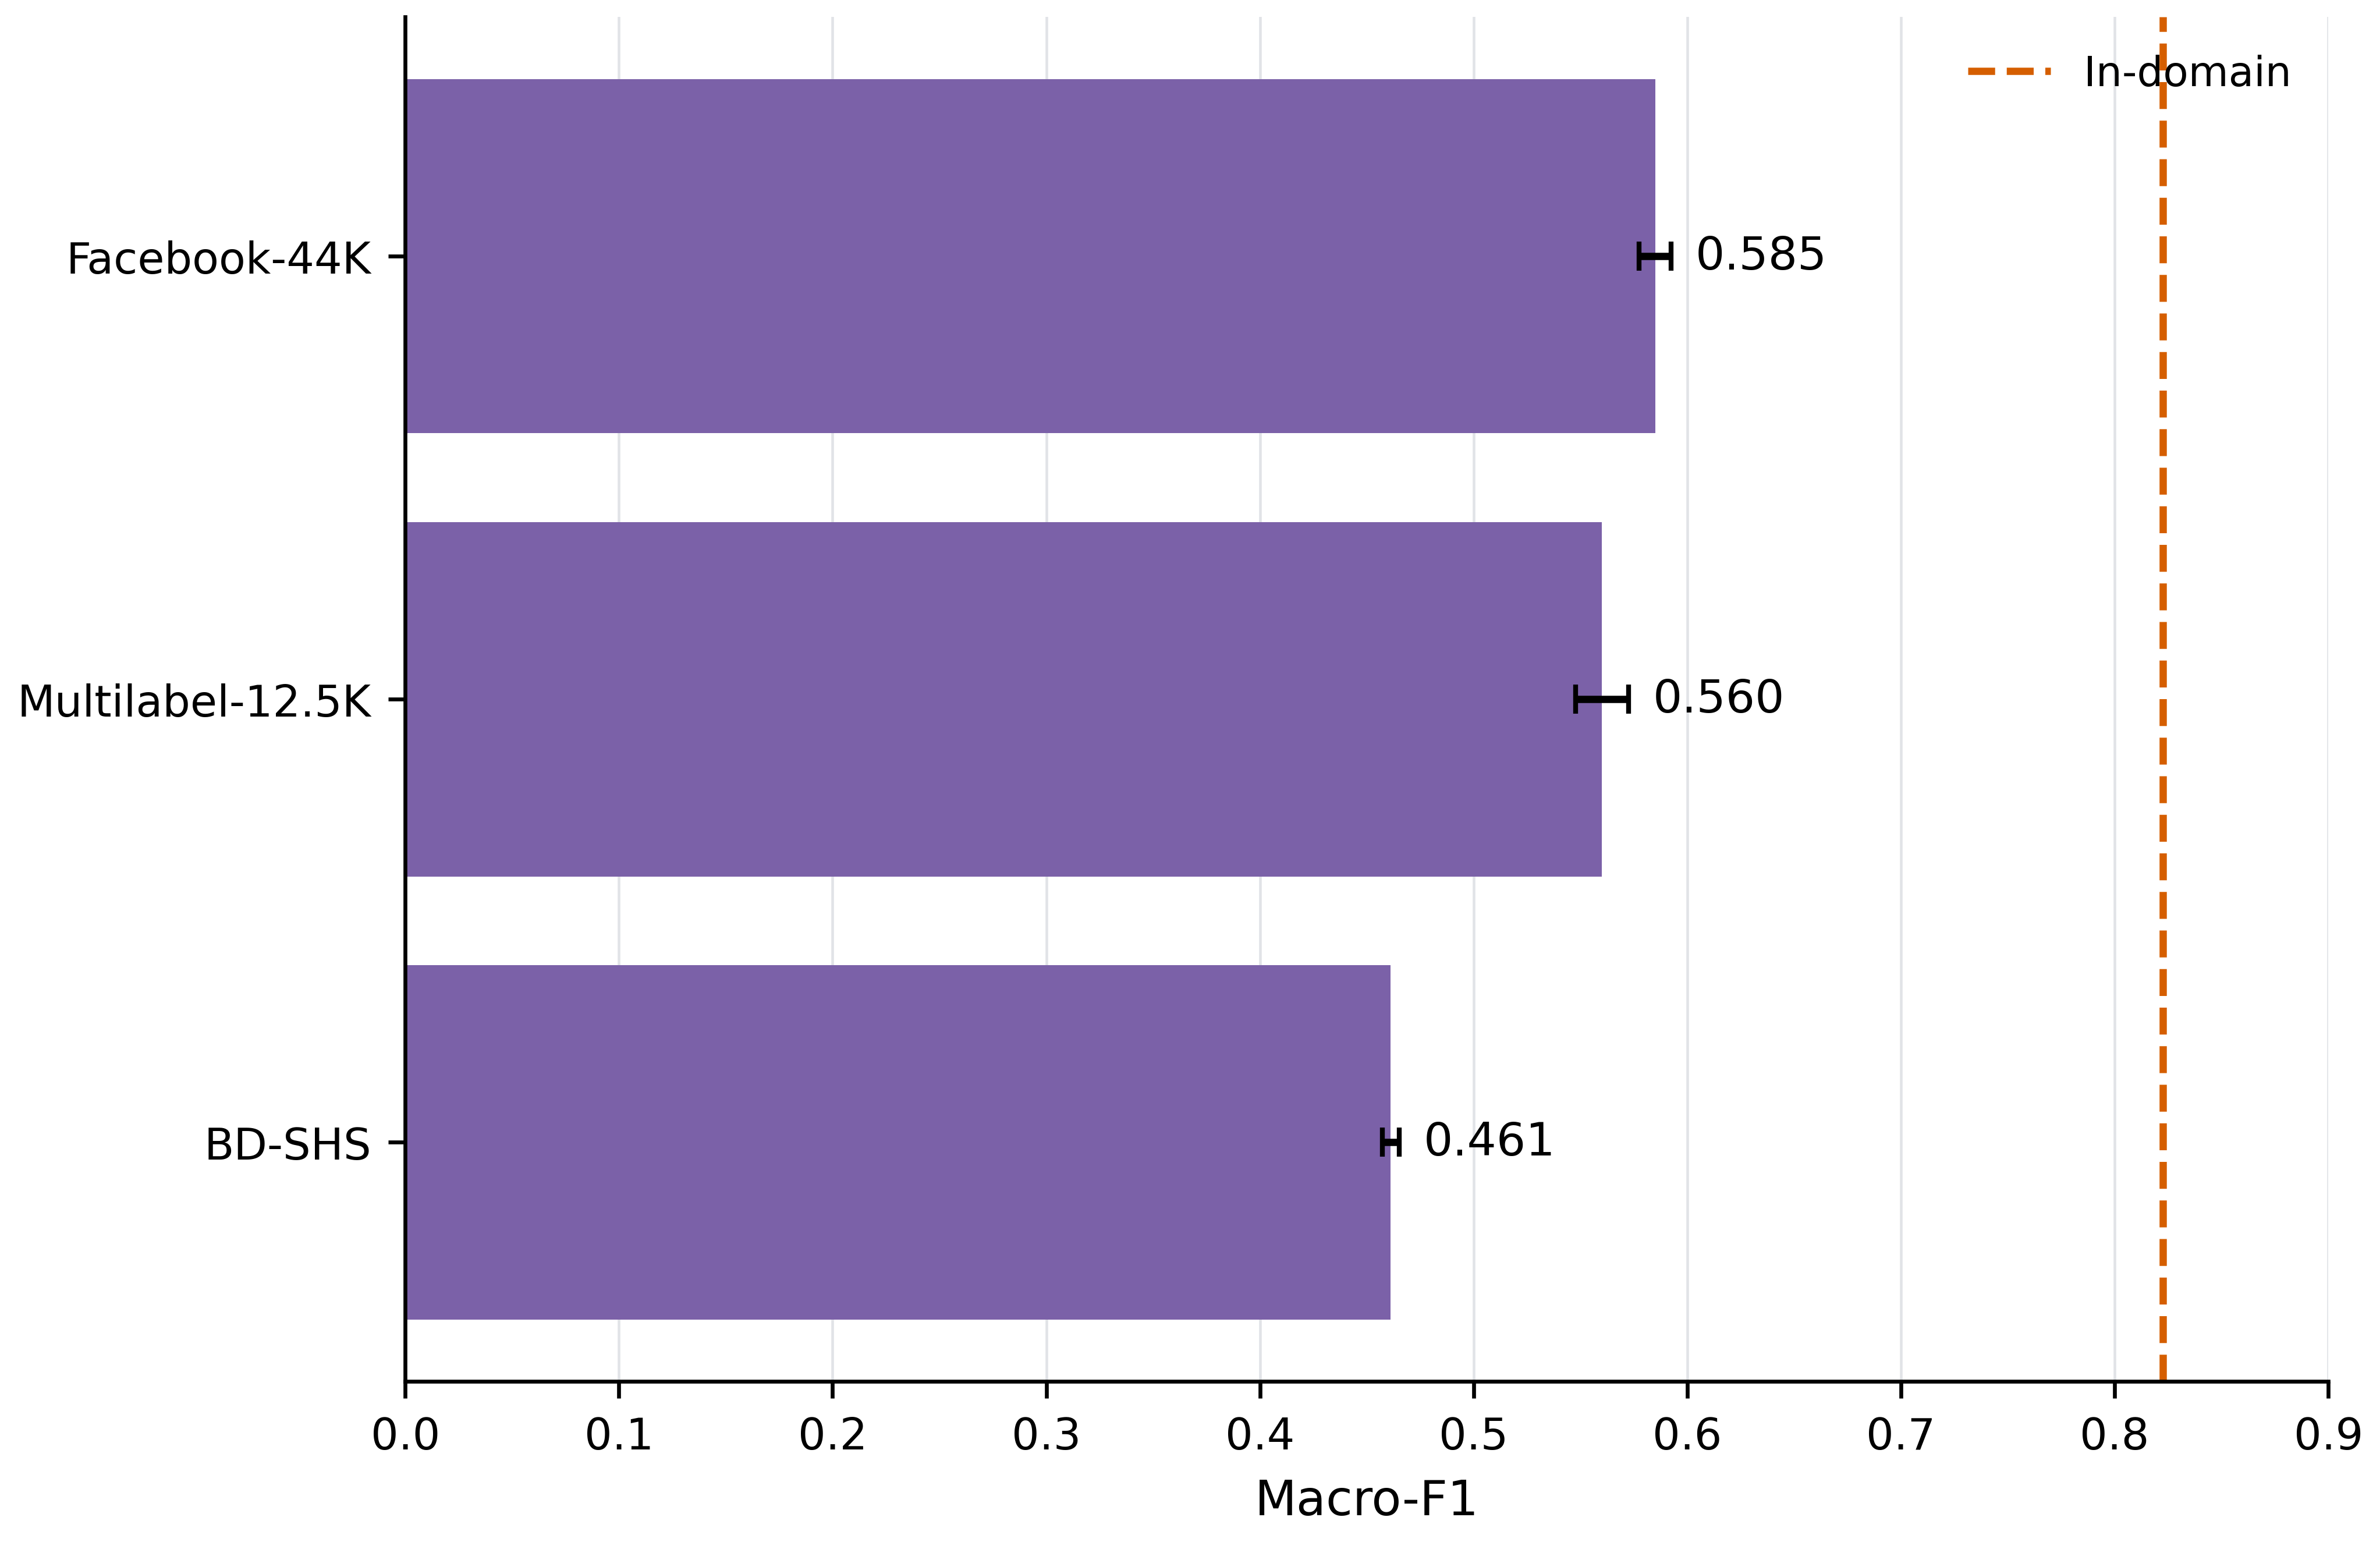
\includegraphics[width=0.72\textwidth]{fig08_robustness.png}
\caption{Source-held-out Macro-F1 (mean $\pm$ std over three seeds) against the in-domain reference (dashed).}
\label{fig:robustness}
\end{figure}

Source-held-out Macro-F1 ranges from 0.4612 to 0.5850, substantially below the in-domain result. The configuration with the smallest training pool does not have the lowest held-out score, so training size alone does not explain the ordering. The held-out sources also differ in class distribution and annotation policy, and the experiment measures their combined effect rather than attributing the difference to one factor. \Cref{tab:holdout-priors} in \cref{sec:appendix} shows substantial class-distribution differences between the training and held-out sets. These differences are one component of the measured source shift, but the experiment does not isolate their effect from language, sampling, or annotation-policy differences. The seed spread is tight, with standard deviations between 0.0039 and 0.0123, which indicates that the observed shift is reproducible for this protocol rather than universal across Bengali corpora. Macro-AUROC remains between 0.83 and 0.87 while Macro-F1 falls. Source-held-out probabilities were not retained, so we do not report expected calibration error or Brier scores for these configurations and we make no calibration claim from AUROC alone. Target-source validation or threshold recalibration is a plausible mitigation, but its effect is not measured here. The practical implication is that in-domain performance should not be treated as evidence of readiness on an unseen source.

\subsection{Comparison with the Base Paper}
\label{sec:basepaper-results}

We retrain the model under the published comparator's protocol: the Facebook-44K source, within-source deduplication, the native five classes (Not Bully, Sexual, Troll, Religious, Threat), and a 70/15/15 split. The comparator evaluates eight pretrained backbones under an ensemble and MLP stacking protocol and does not use FGM, so our row is a protocol-aligned variant with four backbones, cross-entropy with FGM, and our documented preprocessing, rather than a reimplementation of its training procedure. Under this protocol the proposed variant obtains a Macro-F1 of 0.8679, compared with the reported value of 0.8803. Threat F1 is 0.8292 for the proposed variant and 0.8197 in the comparator. The evaluated splits are not identical, so the comparison is descriptive and unpaired (\cref{tab:basepaper}).

\begin{table}[!htbp]
\centering
\caption{Protocol-aligned comparison with the published Facebook-44K results \citep{hoque2025transformerstacking}. The comparison is unpaired because the evaluated splits are not identical.}
\label{tab:basepaper}
\small
\begin{tabular}{@{}lccr@{}}
\toprule
\textbf{Class / Metric} & \textbf{Base paper} & \textbf{Proposed model} & \textbf{$\Delta$} \\
\midrule
Not Bully & 0.9151 & 0.8891 & $-0.0260$ \\
Religious & 0.9374 & 0.9302 & $-0.0072$ \\
Sexual & 0.8845 & 0.8720 & $-0.0125$ \\
Troll & 0.8446 & 0.8192 & $-0.0254$ \\
\textbf{Threat} & 0.8197 & \textbf{0.8292} & $+0.0095$ \\
\midrule
\textbf{Macro-F1} & \textbf{0.8803} & 0.8679 & $-0.0124$ \\
Weighted-F1 & \textbf{0.8923} & 0.8736 & $-0.0187$ \\
Accuracy & NA & 0.8737 & NA \\
MCC & NA & 0.8314 & NA \\
Macro-AUROC & NA & 0.9747 & NA \\
\bottomrule
\end{tabular}
\end{table}

\begin{figure}[!htbp]
\centering
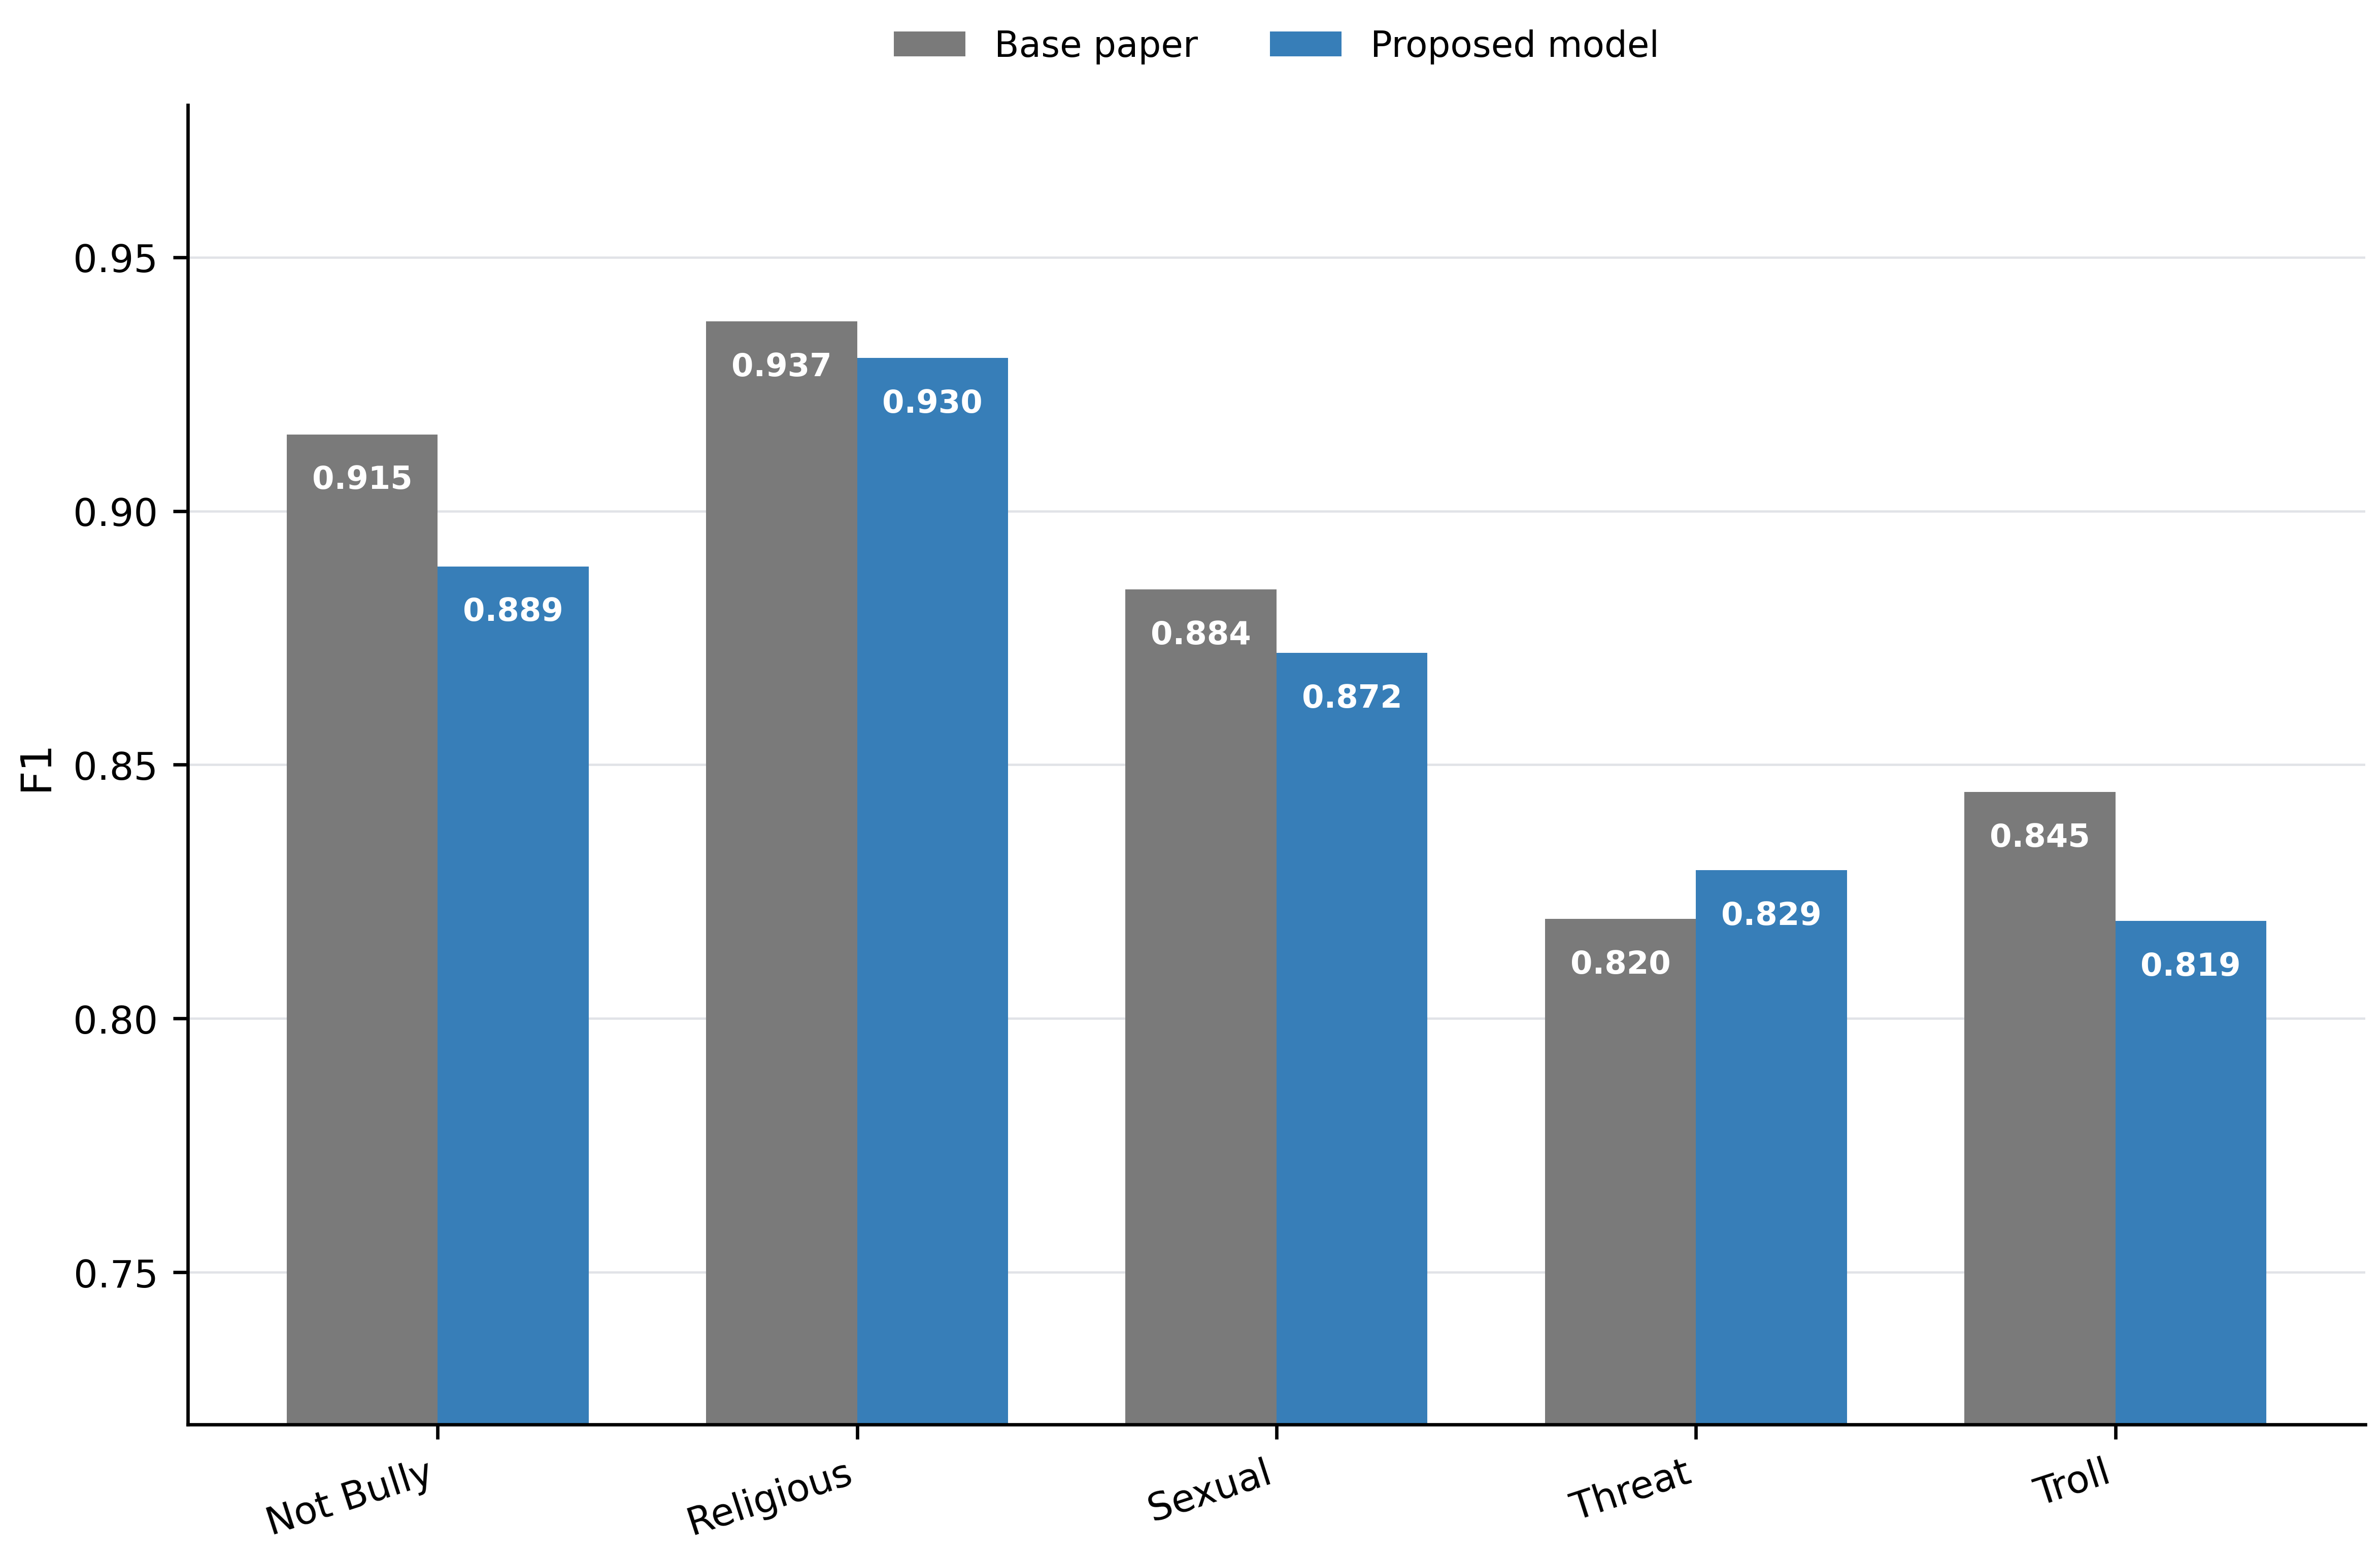
\includegraphics[width=0.78\textwidth]{fig09_basepaper_comparison.png}
\caption{Per-class F1 under the Facebook-44K protocols. Values are descriptive because the evaluated splits are not identical.}
\label{fig:basepaper}
\end{figure}

\Cref{fig:basepaper} plots the per-class values. The proposed variant is 0.0124 below the comparator in Macro-F1 and 0.0095 above it in Threat F1. These are unpaired point estimates under protocol-aligned but non-identical data splits. Our copy of the source carries 43{,}078 comments after within-source deduplication, against the 44{,}001 reported by the comparator, and the published scores are not predictions on our test indices. The two systems also differ in training configuration, since our variant uses cross-entropy with FGM and the comparator does not. We therefore make no claim of statistical superiority or of a new single-dataset state of the art.

\subsection{Ensemble Weights}
\label{sec:ensemble-results}

The selected weights (\cref{fig:weights}) are distributed across several members rather than concentrated on one. Optimized and uniform fusion differ by only 0.0003 Macro-F1 in the retained sensitivity analysis (\cref{tab:fusion}). Weight magnitude therefore should not be interpreted as direct evidence of member quality, error complementarity, or a gain from optimization.

The weights were fitted on the validation split alone under a single non-nested design, constrained to the simplex, and frozen before the test readout. Fitting eleven free parameters on 9{,}432 validation examples carries some risk of validation overfitting, but the fusion-rule sensitivity analysis bounds how much that can matter, since uniform averaging is within 0.0003 of the selected rule. We do not isolate the marginal value of each added backbone and seed, which would require a controlled ensemble-design study.

\begin{figure}[!htbp]
\centering
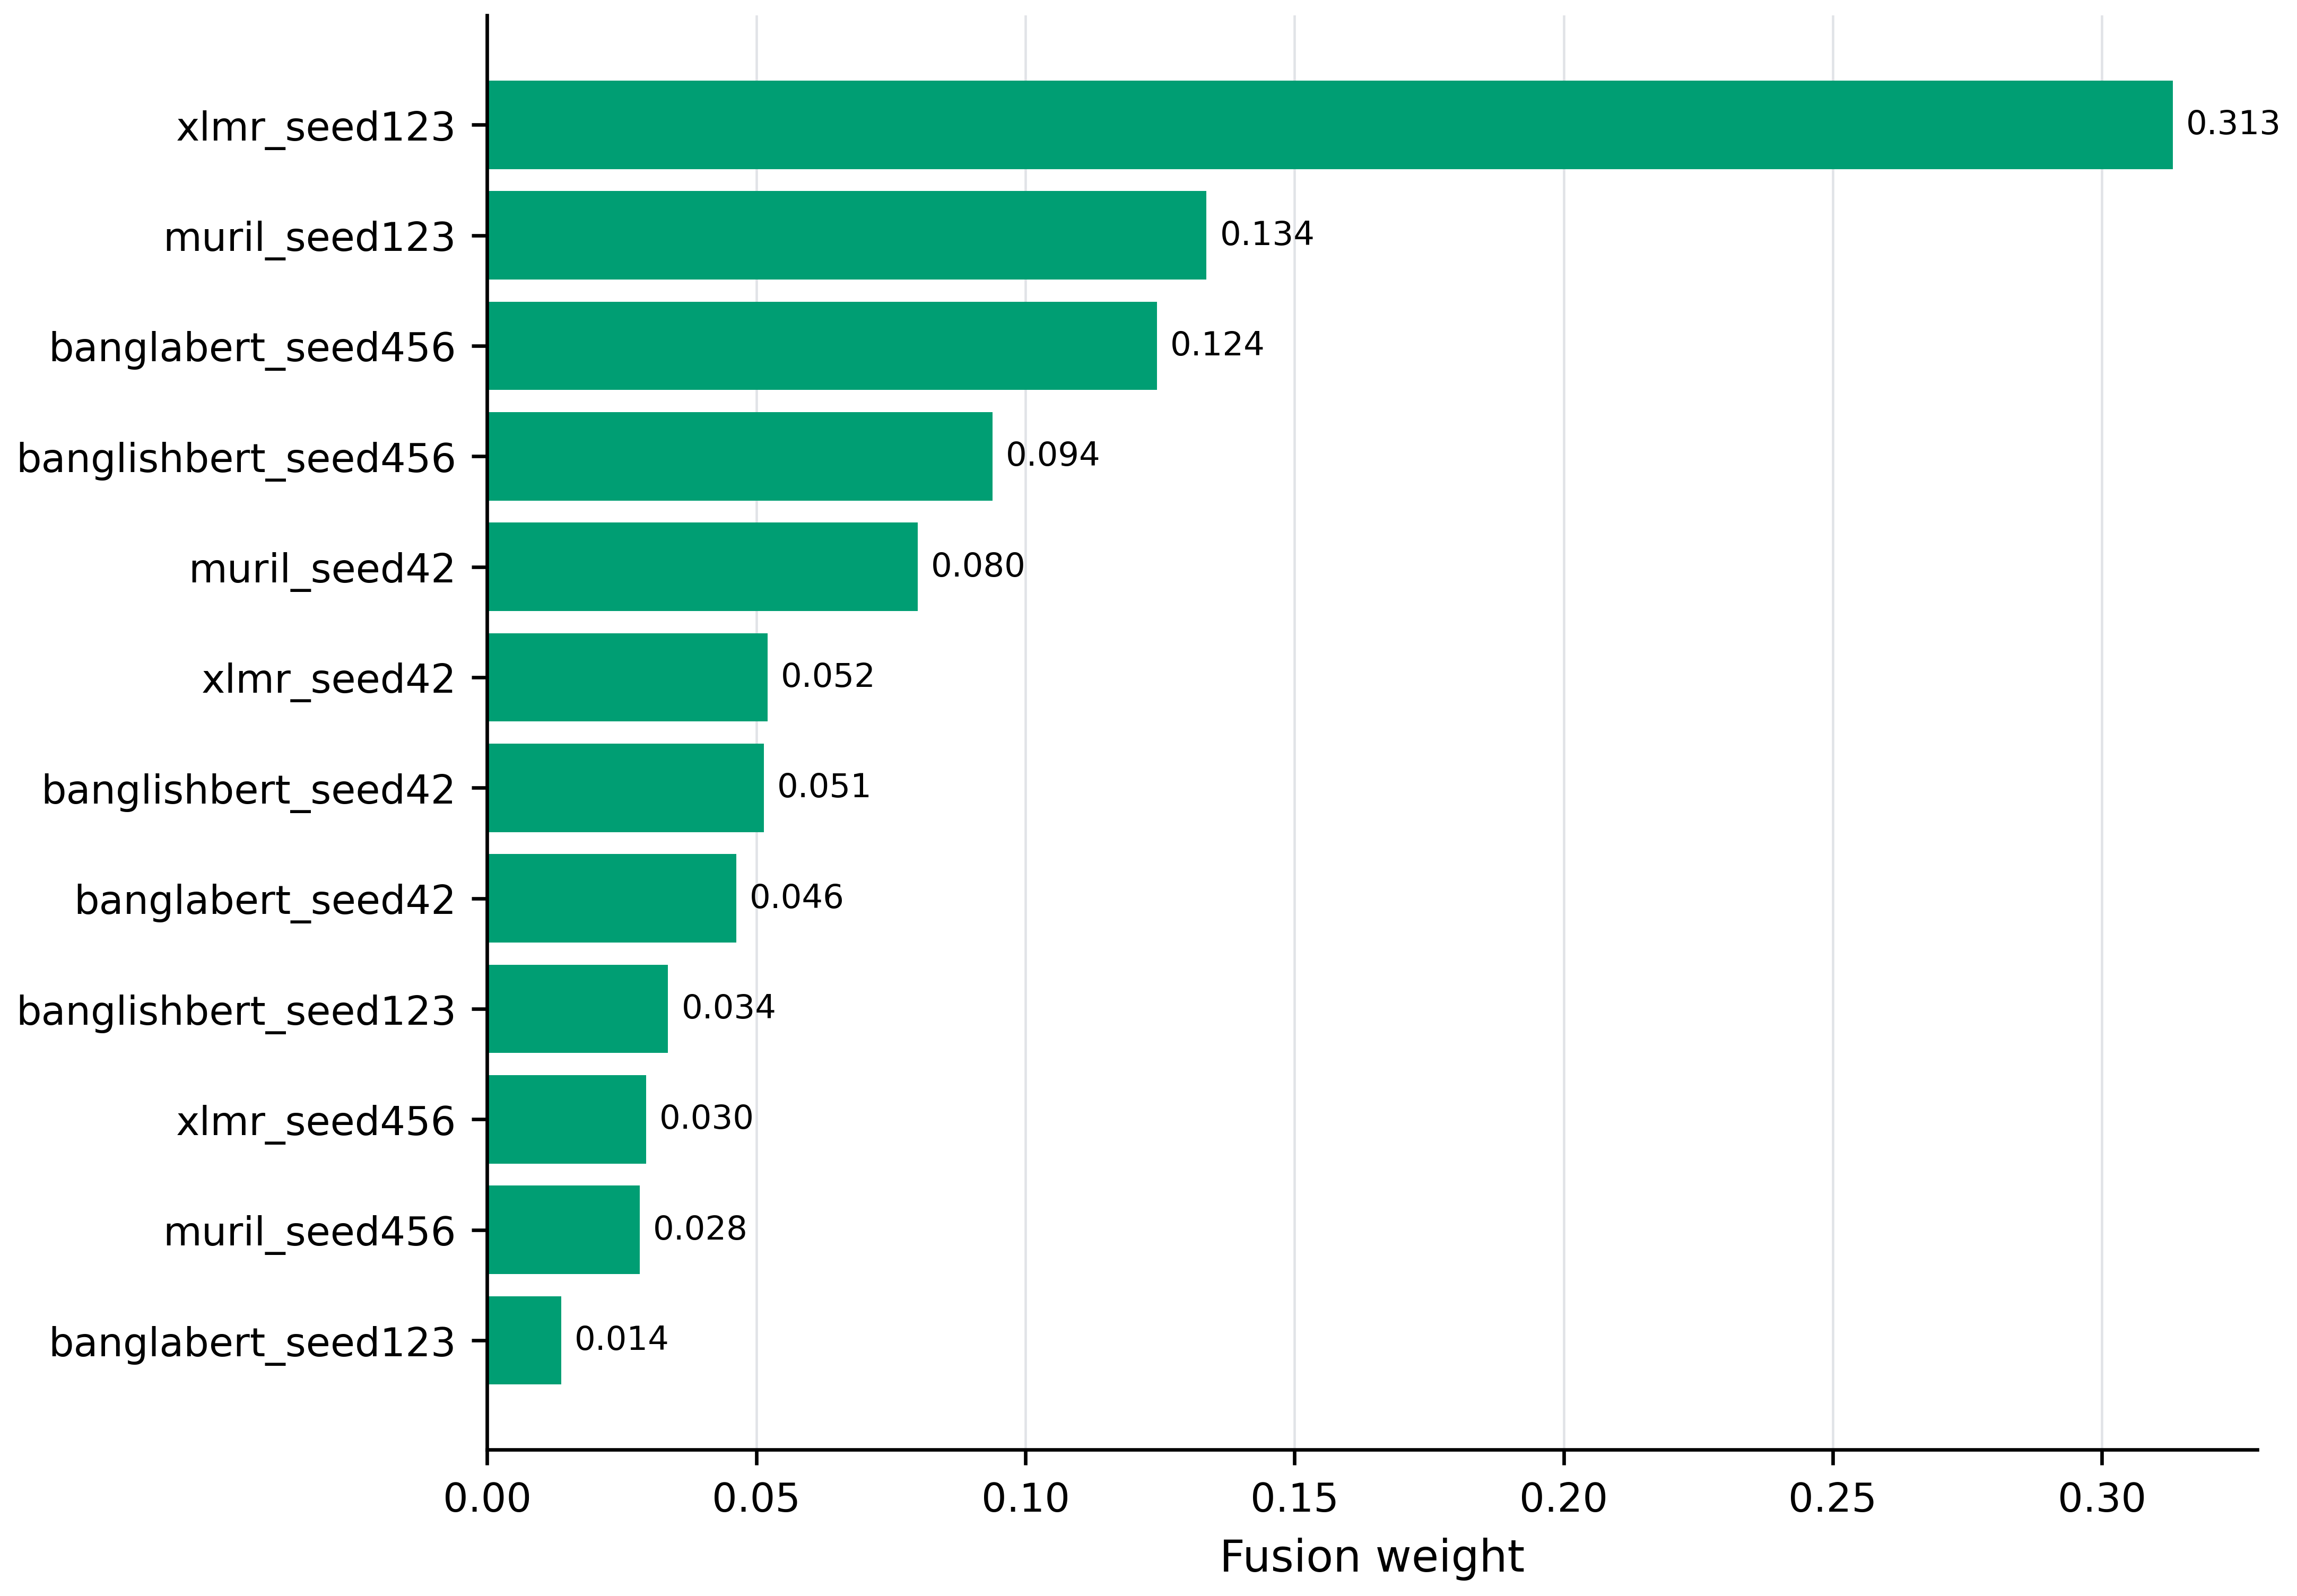
\includegraphics[width=0.72\textwidth]{fig10_ensemble_weights.png}
\caption{Validation-selected fusion weights for the twelve ensemble members.}
\label{fig:weights}
\end{figure}


\section{Discussion}
\label{sec:discussion}

\subsection{What the Results Show}
\label{sec:discussion-together}

In-domain Macro-F1 is 0.8225, while source-held-out Macro-F1 ranges from 0.4612 to 0.5850. FGM produces the largest first point-estimate increase in the component sensitivity study. Script-stratified evaluation shows a lower fixed five-class Macro-F1 for Romanized comments, where Religious and Sexual support is small and Threat support is zero. These results reproduce known cross-dataset degradation in a Bengali setting and show why script-level scores should be reported together with class support.

The routing rule follows from the pretraining scope of the encoders rather than from a measured improvement. BanglaBERT is pretrained primarily on Bangla script, so it is excluded from Romanized inputs, and the bilingual and multilingual encoders remain active on both subsets. The selected fusion weights are distributed across members, but uniform averaging matches the selected rule to within 0.0003 Macro-F1, so the weights are not evidence that individual members contribute different competencies.

Under the comparator's own Facebook-44K protocol, the proposed variant is 0.0124 below the reported Macro-F1 and 0.0095 above the reported Threat F1. Both are unpaired point estimates on non-identical splits. The proposed system is built for four sources and two scripts rather than for one clean single-source corpus, and we make no claim that either difference is statistically established.


\subsection{Limitations and Threats to Validity}
\label{sec:limitations}

Several limitations bound the claims of this study. Script-stratified differences should be interpreted descriptively, because the Romanized comments come from BanTH and the Bangla-script comments come from the other three sources, so script and source are not separable in this benchmark. The Romanized test subset contains only 30 Religious and 51 Sexual examples and no Threat examples, so the corresponding class estimates are unstable and the fixed five-class Romanized Macro-F1 is capped at 0.80 by convention. Paired predictions were not retained for the final member comparison, the routing comparison, or the comparator comparison, so those differences are descriptive rather than tested. Exact-text deduplication does not detect paraphrase-level overlap. Any residual near-duplicate crossing the train and test boundary would inflate the in-domain figure rather than deflate it.

Further limitations concern scope.

These limitations qualify the interpretation of the reported results. They do not invalidate the benchmark construction, and they do not require additional experiments for the present study.


\section{Conclusion and Future Work}
\label{sec:conclusion}

We evaluate a shared five-class Bengali harmful-language benchmark across Bangla and Romanized scripts. \bench{} consolidates four public sources into 94{,}323 comments under a documented taxonomy, and the script-aware ensemble of four encoders is trained with cross-entropy and FGM. The ensemble obtains a Macro-F1 of 0.8225 in-domain with percentile-bootstrap intervals, while source-held-out performance ranges from 0.4612 to 0.5850. Script-stratified results also show lower support for several Romanized minority classes, with no Threat examples at all. These findings support source-held-out and script-stratified reporting with explicit class support for Bengali harmful-language detection.

Future work may retain paired predictions for statistical testing, add further Romanized sources so that script and source effects can be separated, and examine transliteration or cross-script adaptation. A severity-aware or multi-label extension of the taxonomy is also possible once the annotated data can support it. These are future directions rather than requirements for the present study.


\section*{Declarations}

\noindent\textbf{Funding.} This research received no specific grant from any funding agency in the public, commercial, or not-for-profit sectors.

\noindent\textbf{Competing Interests.} The authors declare no competing interests.

\noindent\textbf{Ethical Considerations.} The study uses previously released research datasets and does not collect new social-media data. Two authors annotated an already collected sample for taxonomy validation. The material contains offensive, sexual, religious, and threatening language, so the release carries a content warning. Dataset redistribution and removal procedures must follow the licences and terms of the original sources. The study did not conduct a comprehensive PII or fairness audit.

\noindent\textbf{Data and Code Availability.} Processing code, evaluation code, predictions, split metadata, and permitted research artifacts are available at \url{https://github.com/Sefayet-Alam/BanglaCyberBench}. Source text remains subject to the licences and redistribution terms of the original datasets.

\noindent\textbf{Author Contributions.} S.A.\ led the conceptualisation, methodology, and implementation, ran all training and evaluation, performed the analysis, and wrote the original draft. S.A.\ and N.P.\ carried out the independent label validation and annotation study of \cref{sec:taxonomy}. N.P.\ and A.F.M.M.R.\ contributed to the experimental design, the interpretation of results, and the review and editing of the manuscript. All authors read and approved the final version.

\noindent\textbf{Declaration of Generative AI and AI-assisted Technologies.} The authors used AI-assisted tools only to support software development, debugging, and the scripted generation of result tables and figures. All research design, analysis, interpretation, and manuscript writing were carried out by the authors, who reviewed all outputs and take full responsibility for the content of this publication.

\appendix
\section{Supplementary Tables}
\label{sec:appendix}

\begin{table}[!htbp]
\centering
\caption{Retained non-transformer and neural baseline results on the in-domain test split.}
\label{tab:baseline-full}
\small
\begin{tabular}{@{}lrrrrr@{}}
\toprule
\textbf{System} & \textbf{Macro-F1} & \textbf{Weighted-F1} & \textbf{Accuracy} & \textbf{MCC} & \textbf{Macro-AUROC} \\
\midrule
TF-IDF + logistic regression & 0.5025 & 0.6142 & 0.6025 & 0.4273 & 0.8460 \\
TF-IDF word/character $n$-grams + linear SVM & 0.7674 & 0.7889 & 0.7933 & 0.6788 & 0.9418 \\
BiLSTM & 0.6850 & 0.7106 & 0.7065 & 0.5663 & 0.9052 \\
\bottomrule
\end{tabular}
\end{table}

\begin{table}[!htbp]
\centering
\caption{In-domain ranking and calibration measures by script. Supported AUROC excludes classes with zero gold support in the subset. These are in-domain values and are not source-held-out calibration estimates.}
\label{tab:calibration}
\small
\begin{tabular}{@{}lrrr@{}}
\toprule
\textbf{Subset} & \textbf{Supported AUROC} & \textbf{ECE} & \textbf{Brier score} \\
\midrule
All & 0.9626 & 0.0328 & 0.2482 \\
Bangla & 0.9671 & 0.0348 & 0.2454 \\
Romanized & 0.8743 & 0.0301 & 0.2524 \\
\bottomrule
\end{tabular}
\end{table}

\begin{table}[!htbp]
\centering
\caption{Class shares in the training and held-out test sets for each source-held-out configuration.}
\label{tab:holdout-priors}
\scriptsize
\begin{tabular}{@{}llrrrrr@{}}
\toprule
\textbf{Held-out source} & \textbf{Split} & \textbf{None} & \textbf{Abusive} & \textbf{Religious} & \textbf{Sexual} & \textbf{Threat} \\
\midrule
Facebook-44K & Train & 41.4\% & 31.3\% & 3.3\% & 13.2\% & 10.8\% \\
Facebook-44K & Test  & 34.4\% & 24.1\% & 17.3\% & 20.3\% & 3.9\% \\
Multilabel-12.5K & Train & 36.3\% & 24.1\% & 15.7\% & 19.0\% & 5.0\% \\
Multilabel-12.5K & Test  & 35.5\% & 35.4\% & 4.1\% & 16.5\% & 8.6\% \\
BD-SHS & Train & 34.6\% & 26.0\% & 15.0\% & 19.7\% & 4.7\% \\
BD-SHS & Test  & 51.8\% & 24.0\% & 2.0\% & 7.4\% & 14.7\% \\
\bottomrule
\end{tabular}
\end{table}


{\footnotesize
\bibliography{References}}

\end{document}